\documentclass[aspectratio=169,11pt]{beamer}
% ==========================================================================
%  KSA lecture-slide theme  =  stock beamer "Boadilla"  +  KSA colour theme
%  brand colours sampled from the official KSA symbol mark:
%    Deep Prussian Blue  #2E3192   (지성 - intellect)
%    Golden Gray         #D6CBB1   (감성 - sensibility)
%  Engine: XeLaTeX.  Usage:
%    \documentclass[aspectratio=169,11pt]{beamer}
%    % ==========================================================================
%  KSA lecture-slide theme  =  stock beamer "Boadilla"  +  KSA colour theme
%  brand colours sampled from the official KSA symbol mark:
%    Deep Prussian Blue  #2E3192   (지성 - intellect)
%    Golden Gray         #D6CBB1   (감성 - sensibility)
%  Engine: XeLaTeX.  Usage:
%    \documentclass[aspectratio=169,11pt]{beamer}
%    % ==========================================================================
%  KSA lecture-slide theme  =  stock beamer "Boadilla"  +  KSA colour theme
%  brand colours sampled from the official KSA symbol mark:
%    Deep Prussian Blue  #2E3192   (지성 - intellect)
%    Golden Gray         #D6CBB1   (감성 - sensibility)
%  Engine: XeLaTeX.  Usage:
%    \documentclass[aspectratio=169,11pt]{beamer}
%    \input{../theme/ksa-theme.tex}
% ==========================================================================

\usepackage{fontspec}
\usepackage{amsmath,amssymb}
\usepackage{graphicx}
\graphicspath{{figs/}{../figs/}}
\usepackage{booktabs}
\usepackage{listings}

% ---- fonts (no ctex/xeCJK on this box -> fontspec drives CJK directly) -----
\defaultfontfeatures{Ligatures=TeX}
\setmainfont{Noto Sans CJK KR}
\setsansfont{Noto Sans CJK KR}
\setmonofont{Noto Sans Mono CJK KR}[Scale=0.92]

% ---- base theme: stock Boadilla ------------------------------------------
\usetheme{Boadilla}
\usefonttheme{professionalfonts}
\setbeamertemplate{navigation symbols}{}

% ---- KSA colour theme (recolour the stock theme) --------------------------
\definecolor{ksablue}{HTML}{2E3192}
\definecolor{ksabluedk}{HTML}{20226A}
\definecolor{ksagold}{HTML}{D6CBB1}
\definecolor{ksagolddk}{HTML}{A9976B}
\definecolor{ksared}{HTML}{C0392B}
\definecolor{ksagray}{HTML}{5B5B5B}

\setbeamercolor{structure}{fg=ksablue}
\setbeamercolor{alerted text}{fg=ksared}

\setbeamercolor{palette primary}{fg=white,           bg=ksablue}
\setbeamercolor{palette secondary}{fg=white,         bg=ksablue!85!black}
\setbeamercolor{palette tertiary}{fg=white,          bg=ksabluedk}
\setbeamercolor{titlelike}{fg=ksablue}
\setbeamercolor{frametitle}{fg=ksablue,bg=}
\setbeamercolor{title}{fg=ksablue}
\setbeamercolor{author}{fg=ksagray}
\setbeamercolor{institute}{fg=ksagray}
\setbeamercolor{block title}{fg=white,bg=ksablue}
\setbeamercolor{block body}{fg=black!85,bg=ksablue!6}
\setbeamercolor{item}{fg=ksablue}
\setbeamercolor{section in toc}{fg=black!85}

\setbeamerfont{frametitle}{series=\bfseries}
\setbeamerfont{title}{series=\bfseries}

% ---- footline:  KSA mark | "Made by ..." | n / N   (matches reference) ----
\newcommand{\ksacredit}{Made by Sumin Han \,\textperiodcentered\, suminhan@ksa.hs.kr}
\setbeamertemplate{footline}{%
  \hbox{%
    \begin{beamercolorbox}[wd=.18\paperwidth,ht=2.6ex,dp=1.5ex,leftskip=1.1em]{}%
      \raisebox{-0.35ex}{
\includegraphics[height=2.0ex]{ksa-logo.png}}%
    \end{beamercolorbox}%
    \begin{beamercolorbox}[wd=.64\paperwidth,ht=2.6ex,dp=1.5ex,center]{}%
      {\scriptsize\color{ksagray}\ksacredit}%
    \end{beamercolorbox}%
    \begin{beamercolorbox}[wd=.18\paperwidth,ht=2.6ex,dp=1.5ex,rightskip=1.1em]{}%
      \hfill{\scriptsize\color{ksablue}\insertframenumber\,/\,\inserttotalframenumber}%
    \end{beamercolorbox}%
  }%
  \vskip2pt
}

% ---- section divider: stock \sectionpage, KSA-coloured -------------------
\setbeamertemplate{section page}{%
  \begingroup\centering
    {\color{ksagolddk}\rule{0.16\paperwidth}{1pt}}\par\vskip1.0em
    {\usebeamerfont{title}\color{ksablue}\insertsectionhead\par}\vskip1.0em
    {\color{ksagolddk}\rule{0.16\paperwidth}{1pt}}\par
  \endgroup
}
\AtBeginSection[]{\begin{frame}[plain,noframenumbering]\vfill\sectionpage\vfill\end{frame}}

% ---- code listings ------------------------------------------------------------
\lstdefinestyle{ksa}{%
  basicstyle=\ttfamily\scriptsize,
  keywordstyle=\color{ksablue}\bfseries,
  commentstyle=\color{ksagray}\itshape,
  stringstyle=\color{ksagolddk},
  numberstyle=\tiny\color{ksagray},
  backgroundcolor=\color{ksablue!6},
  frame=leftline, framerule=1.4pt, rulecolor=\color{ksablue},
  xleftmargin=1em, aboveskip=0.8em, belowskip=0.4em,
  showstringspaces=false, breaklines=true, language=Python,
}
\lstset{style=ksa}

% ---- handy macros -----------------------------------------------------------
\newcommand{\kb}[1]{\textbf{\color{ksablue}#1}}   % blue keyword
\newcommand{\kq}[1]{\textbf{\color{ksared}#1}}    % red key-question

% ==========================================================================

\usepackage{fontspec}
\usepackage{amsmath,amssymb}
\usepackage{graphicx}
\graphicspath{{figs/}{../figs/}}
\usepackage{booktabs}
\usepackage{listings}

% ---- fonts (no ctex/xeCJK on this box -> fontspec drives CJK directly) -----
\defaultfontfeatures{Ligatures=TeX}
\setmainfont{Noto Sans CJK KR}
\setsansfont{Noto Sans CJK KR}
\setmonofont{Noto Sans Mono CJK KR}[Scale=0.92]

% ---- base theme: stock Boadilla ------------------------------------------
\usetheme{Boadilla}
\usefonttheme{professionalfonts}
\setbeamertemplate{navigation symbols}{}

% ---- KSA colour theme (recolour the stock theme) --------------------------
\definecolor{ksablue}{HTML}{2E3192}
\definecolor{ksabluedk}{HTML}{20226A}
\definecolor{ksagold}{HTML}{D6CBB1}
\definecolor{ksagolddk}{HTML}{A9976B}
\definecolor{ksared}{HTML}{C0392B}
\definecolor{ksagray}{HTML}{5B5B5B}

\setbeamercolor{structure}{fg=ksablue}
\setbeamercolor{alerted text}{fg=ksared}

\setbeamercolor{palette primary}{fg=white,           bg=ksablue}
\setbeamercolor{palette secondary}{fg=white,         bg=ksablue!85!black}
\setbeamercolor{palette tertiary}{fg=white,          bg=ksabluedk}
\setbeamercolor{titlelike}{fg=ksablue}
\setbeamercolor{frametitle}{fg=ksablue,bg=}
\setbeamercolor{title}{fg=ksablue}
\setbeamercolor{author}{fg=ksagray}
\setbeamercolor{institute}{fg=ksagray}
\setbeamercolor{block title}{fg=white,bg=ksablue}
\setbeamercolor{block body}{fg=black!85,bg=ksablue!6}
\setbeamercolor{item}{fg=ksablue}
\setbeamercolor{section in toc}{fg=black!85}

\setbeamerfont{frametitle}{series=\bfseries}
\setbeamerfont{title}{series=\bfseries}

% ---- footline:  KSA mark | "Made by ..." | n / N   (matches reference) ----
\newcommand{\ksacredit}{Made by Sumin Han \,\textperiodcentered\, suminhan@ksa.hs.kr}
\setbeamertemplate{footline}{%
  \hbox{%
    \begin{beamercolorbox}[wd=.18\paperwidth,ht=2.6ex,dp=1.5ex,leftskip=1.1em]{}%
      \raisebox{-0.35ex}{
\includegraphics[height=2.0ex]{ksa-logo.png}}%
    \end{beamercolorbox}%
    \begin{beamercolorbox}[wd=.64\paperwidth,ht=2.6ex,dp=1.5ex,center]{}%
      {\scriptsize\color{ksagray}\ksacredit}%
    \end{beamercolorbox}%
    \begin{beamercolorbox}[wd=.18\paperwidth,ht=2.6ex,dp=1.5ex,rightskip=1.1em]{}%
      \hfill{\scriptsize\color{ksablue}\insertframenumber\,/\,\inserttotalframenumber}%
    \end{beamercolorbox}%
  }%
  \vskip2pt
}

% ---- section divider: stock \sectionpage, KSA-coloured -------------------
\setbeamertemplate{section page}{%
  \begingroup\centering
    {\color{ksagolddk}\rule{0.16\paperwidth}{1pt}}\par\vskip1.0em
    {\usebeamerfont{title}\color{ksablue}\insertsectionhead\par}\vskip1.0em
    {\color{ksagolddk}\rule{0.16\paperwidth}{1pt}}\par
  \endgroup
}
\AtBeginSection[]{\begin{frame}[plain,noframenumbering]\vfill\sectionpage\vfill\end{frame}}

% ---- code listings ------------------------------------------------------------
\lstdefinestyle{ksa}{%
  basicstyle=\ttfamily\scriptsize,
  keywordstyle=\color{ksablue}\bfseries,
  commentstyle=\color{ksagray}\itshape,
  stringstyle=\color{ksagolddk},
  numberstyle=\tiny\color{ksagray},
  backgroundcolor=\color{ksablue!6},
  frame=leftline, framerule=1.4pt, rulecolor=\color{ksablue},
  xleftmargin=1em, aboveskip=0.8em, belowskip=0.4em,
  showstringspaces=false, breaklines=true, language=Python,
}
\lstset{style=ksa}

% ---- handy macros -----------------------------------------------------------
\newcommand{\kb}[1]{\textbf{\color{ksablue}#1}}   % blue keyword
\newcommand{\kq}[1]{\textbf{\color{ksared}#1}}    % red key-question

% ==========================================================================

\usepackage{fontspec}
\usepackage{amsmath,amssymb}
\usepackage{graphicx}
\graphicspath{{figs/}{../figs/}}
\usepackage{booktabs}
\usepackage{listings}

% ---- fonts (no ctex/xeCJK on this box -> fontspec drives CJK directly) -----
\defaultfontfeatures{Ligatures=TeX}
\setmainfont{Noto Sans CJK KR}
\setsansfont{Noto Sans CJK KR}
\setmonofont{Noto Sans Mono CJK KR}[Scale=0.92]

% ---- base theme: stock Boadilla ------------------------------------------
\usetheme{Boadilla}
\usefonttheme{professionalfonts}
\setbeamertemplate{navigation symbols}{}

% ---- KSA colour theme (recolour the stock theme) --------------------------
\definecolor{ksablue}{HTML}{2E3192}
\definecolor{ksabluedk}{HTML}{20226A}
\definecolor{ksagold}{HTML}{D6CBB1}
\definecolor{ksagolddk}{HTML}{A9976B}
\definecolor{ksared}{HTML}{C0392B}
\definecolor{ksagray}{HTML}{5B5B5B}

\setbeamercolor{structure}{fg=ksablue}
\setbeamercolor{alerted text}{fg=ksared}

\setbeamercolor{palette primary}{fg=white,           bg=ksablue}
\setbeamercolor{palette secondary}{fg=white,         bg=ksablue!85!black}
\setbeamercolor{palette tertiary}{fg=white,          bg=ksabluedk}
\setbeamercolor{titlelike}{fg=ksablue}
\setbeamercolor{frametitle}{fg=ksablue,bg=}
\setbeamercolor{title}{fg=ksablue}
\setbeamercolor{author}{fg=ksagray}
\setbeamercolor{institute}{fg=ksagray}
\setbeamercolor{block title}{fg=white,bg=ksablue}
\setbeamercolor{block body}{fg=black!85,bg=ksablue!6}
\setbeamercolor{item}{fg=ksablue}
\setbeamercolor{section in toc}{fg=black!85}

\setbeamerfont{frametitle}{series=\bfseries}
\setbeamerfont{title}{series=\bfseries}

% ---- footline:  KSA mark | "Made by ..." | n / N   (matches reference) ----
\newcommand{\ksacredit}{Made by Sumin Han \,\textperiodcentered\, suminhan@ksa.hs.kr}
\setbeamertemplate{footline}{%
  \hbox{%
    \begin{beamercolorbox}[wd=.18\paperwidth,ht=2.6ex,dp=1.5ex,leftskip=1.1em]{}%
      \raisebox{-0.35ex}{
\includegraphics[height=2.0ex]{ksa-logo.png}}%
    \end{beamercolorbox}%
    \begin{beamercolorbox}[wd=.64\paperwidth,ht=2.6ex,dp=1.5ex,center]{}%
      {\scriptsize\color{ksagray}\ksacredit}%
    \end{beamercolorbox}%
    \begin{beamercolorbox}[wd=.18\paperwidth,ht=2.6ex,dp=1.5ex,rightskip=1.1em]{}%
      \hfill{\scriptsize\color{ksablue}\insertframenumber\,/\,\inserttotalframenumber}%
    \end{beamercolorbox}%
  }%
  \vskip2pt
}

% ---- section divider: stock \sectionpage, KSA-coloured -------------------
\setbeamertemplate{section page}{%
  \begingroup\centering
    {\color{ksagolddk}\rule{0.16\paperwidth}{1pt}}\par\vskip1.0em
    {\usebeamerfont{title}\color{ksablue}\insertsectionhead\par}\vskip1.0em
    {\color{ksagolddk}\rule{0.16\paperwidth}{1pt}}\par
  \endgroup
}
\AtBeginSection[]{\begin{frame}[plain,noframenumbering]\vfill\sectionpage\vfill\end{frame}}

% ---- code listings ------------------------------------------------------------
\lstdefinestyle{ksa}{%
  basicstyle=\ttfamily\scriptsize,
  keywordstyle=\color{ksablue}\bfseries,
  commentstyle=\color{ksagray}\itshape,
  stringstyle=\color{ksagolddk},
  numberstyle=\tiny\color{ksagray},
  backgroundcolor=\color{ksablue!6},
  frame=leftline, framerule=1.4pt, rulecolor=\color{ksablue},
  xleftmargin=1em, aboveskip=0.8em, belowskip=0.4em,
  showstringspaces=false, breaklines=true, language=Python,
}
\lstset{style=ksa}

% ---- handy macros -----------------------------------------------------------
\newcommand{\kb}[1]{\textbf{\color{ksablue}#1}}   % blue keyword
\newcommand{\kq}[1]{\textbf{\color{ksared}#1}}    % red key-question


\title{Block A 캡스톤: 팀 프로젝트와 총정리}
\subtitle{팀 프로젝트 구조와 발표 \,$\cdot$\, Peer-Review \,$\cdot$\, 중간고사 대비}
\author{Machine Learning 2 \,\textperiodcentered\, 8주차}
\institute{한국과학영재학교 (KSA)}
\date{Chapter 8}

\begin{document}

% ===== title =====
\begin{frame}[plain,noframenumbering]
  \titlepage
\end{frame}

% ===== roadmap of this week =====
\begin{frame}{이번 주차 개요}
  \begin{itemize}
    \item Chapter 2$\sim$7: 밴딧, MDP, DP, MC, TD, n-step ---
      \kb{표 기반(tabular) 강화학습 이론 전체}를 훑었다.
    \item 이번 장은 \textbf{새 개념 0개} --- 그 이론을 Gymnasium의 표 기반
      환경에서 \textbf{직접 구현·비교}하고, 중간고사를 준비하는 장.
    \item \kb{역전}: 환경·알고리즘·시드를 고르는 것, 그리고 \textbf{심사자가
      되는 것}까지가 이번 주.
  \end{itemize}
  \vskip0.6em
  \begin{block}{이 챕터를 마치면}
    \begin{itemize}
      \item 두 개 이상 알고리즘을 \textbf{시드 $\geq 3$ + greedy
        ($\varepsilon=0$) 평가 분리} 프로토콜로 비교·보고 (8.1).
      \item 결과를 Ch\,2$\sim$7 개념(on/off-policy, 편향-분산)으로
        \textbf{수식적으로 정당화}, 잘 안 된 부분까지 숨기지 않고 진단 (8.1).
      \item 4항목 체크리스트로 다른 팀 발표를 심사, \textbf{3점(반박 가능한)
        질문}을 작성 (8.2).
      \item 손유도 템플릿 3종의 빈칸을 스스로 채우고, 20문항 자가진단으로
        준비도를 재봄 (8.3).
    \end{itemize}
  \end{block}
\end{frame}

\section{8.1 팀 프로젝트: 구조와 발표}

\begin{frame}{왜 지금 프로젝트를 하는가}
  \begin{itemize}
    \item Ch\,2$\sim$7: 밴딧 $\to$ n-step TD·Dyna-Q까지 표 기반 RL 이론을
      손에 쥨 --- Sutton \& Barto 표준 교과서와 거의 1:1.
    \item 지금까지 해본 것: \textbf{``교재가 고른 환경, 교재가 고른
      파라미터, 교재가 고른 시드''}에서 코드가 동작하는지 확인.
    \item 지금 필요한 것: 한 단계 위로 --- \textbf{환경을 고르고, 알고리즘
      두 개를 고르고, 결과가 흔들리면 시드와 프로토콜을 점검해서 다시
      고르는 것}까지.
    \item ``코드가 동작한다''는 증거 $\neq$ ``이 문제를 내가 설계하고
      평가할 수 있다''는 증거.
  \end{itemize}
  \vskip0.6em
  \begin{block}{프로젝트를 마치면 손에 넣는 것}
    보고서 + 발표 + peer-review --- ``설계하고 평가할 수 있다''의 증거.
  \end{block}
\end{frame}

\begin{frame}{프로젝트 구조: 환경 · 2개 이상 알고리즘 · 필수 요구사항}
  \begin{itemize}
    \item \kb{환경}: Gymnasium의 \textbf{표 기반(이산 상태·행동)} 환경 하나 ---
      \texttt{FrozenLake-v1}, \texttt{CliffWalking-v1}, \texttt{Taxi-v4} 등.
    \item \kb{적용}: Ch\,4$\sim$7 알고리즘 \textbf{최소 두 가지}를 같은 환경에
      적용 (예: Q-learning vs SARSA, MC 제어 vs n-step TD) $\to$ 학습 곡선과
      최종 정책 비교.
    \item \kb{필수 --- 수식적 정당화 최소 1개}:
    \begin{itemize}
      \item Q-learning/SARSA 비교 $\to$ Ch\,6.2$\sim$6.3 on/off-policy로
        정책이 왜 다르게 학습됐는지 설명.
      \item $\varepsilon$/$\alpha$ 변경 실험 $\to$ Ch\,6.3 수렴 조건과 연결.
      \item Dyna-Q 사용 $\to$ Ch\,7.3 계획 스텝 수와 학습 속도를 \textbf{직접 측정}.
    \end{itemize}
  \end{itemize}
\end{frame}

\begin{frame}{환경 고르는 실전 가이드: 점수를 매기는 4가지 기준}
  \small
  \begin{tabular}{@{}p{0.28\textwidth}p{0.66\textwidth}@{}}
    \toprule
    기준 & 왜인가 \\
    \midrule
    (1) 상태-행동 공간 크기 & 상태가 많으면(Taxi 500개) 표를 채우는
      에피소드 수가 급증 \\
    (2) 보상 구조가 ``학습 중''과 ``최종 정책''을 갈라놓나 & CliffWalking처럼
      실수에 비례하지 않게 큰 벌($-100$) $\to$ on/off-policy 차이가 극적으로
      드러나 6.3절을 숫자로 보여줌 \\
    (3) 확률적 전이 & FrozenLake 미끄럼 $\to$ ``같은 정책이어도 에피소드가
      매번 달라지는'' RL 특유의 불확실성 체감 \\
    (4) 코드 재사용성 & Ch\,6.3·7.3 강의 코드가 거의 그대로 적용되는가.
      시작 상태 다중 여부(Taxi)·에피소드 길이 상한 확인 \\
    \bottomrule
  \end{tabular}
  \vskip0.8em
  {\footnotesize Gymnasium 레지스트리 이름은 버전에 따라 달라짐 --- 최근 버전에서
  \texttt{Taxi-v3}는 deprecated $\to$ \texttt{Taxi-v4} 사용.
  CliffWalking은 \texttt{gym.make("CliffWalking-v1")} 로 바로 사용
  (4$\times$12 격자, 시작=좌하단, 목표=우하단, 사이를 절벽이 가로막음).}
\end{frame}

\begin{frame}{후보 환경 비교표}
  \scriptsize
  \begin{tabular}{@{}p{0.17\textwidth}p{0.15\textwidth}p{0.30\textwidth}cp{0.30\textwidth}@{}}
    \toprule
    환경 & 상태$\times$행동 & 보상 구조 & 난이도 & 잘 어울리는 비교 \\
    \midrule
    \textbf{FrozenLake-v1} & 16$\times$4 (미끄럼) & 도착 +1, 그 외 0
      (구멍=종료) & 낮 & MC(Ch\,5.3) vs SARSA(Ch\,6.3) --- 확률 전이에서
      시드 안정성 \\
    \textbf{CliffWalking-v1} & 48$\times$4 & 스텝 $-1$, 절벽 $-100$,
      도착 0 & 중 & SARSA vs Q-learning --- 6.3절의 클래식 비교 \\
    \textbf{Taxi-v4} & 500$\times$6 & 성공 +20, 불법 $-10$, 스텝 $-1$ & 높 &
      n-step vs TD(0) (Ch\,7.2), Dyna-Q (Ch\,7.3) \\
    \bottomrule
  \end{tabular}
  \vskip1em
  \begin{block}{선택은 자유이지만}
    선택이 \textbf{Ch\,4$\sim$7의 개념 검증 목적}에 근거해야 한다.
    (상태 수 · 보상 구조 · 확률 전이 중 무엇이 이 비교를 정당화하는지)
  \end{block}
\end{frame}

\begin{frame}{비교 프로토콜 (1/3): 시드 $\geq 3$ --- 왜인가}
  \begin{itemize}
    \item ``한 번의 실행''은 아무것도 말해주지 않는다:
    \begin{itemize}
      \item $\varepsilon$-greedy 탐험의 무작위성,
      \item (FrozenLake처럼) \textbf{환경 전이 자체}의 무작위성,
      \item 정책 초기화.
    \end{itemize}
    \item $\to$ \textbf{같은 코드·같은 파라미터를 그대로 돌려도 매번 다른
      학습 곡선}이 나온다.
    \item \kb{시드를 바꾸는 것}은 ``실험을 다시 하는 것''이 아니라
      \textbf{``우연에 좌우되는지 재검사하는 것''}.
  \end{itemize}
  \vskip0.6em
  \begin{block}{프로토콜의 세 규칙}
    \begin{enumerate}
      \item \textbf{시드 $\geq 3$} (예: 0, 1, 2)으로 알고리즘을 \textbf{전부
        다시} 학습.
      \item \textbf{학습 도중 성과}와 \textbf{학습 후 평가 성과}를 반드시
        \textbf{분리}해 보고.
      \item 비교는 \textbf{시드별 숫자 자체}(예: ``$-13$ / $-13$ / $-13$'')를
        표로 제시하고, 평균$\pm$표준편차나 ``일관된 경향''으로 결론.
    \end{enumerate}
  \end{block}
\end{frame}

\begin{frame}{비교 프로토콜 (2/3): 학습 중 리턴 vs 학습 후 평가}
  \begin{columns}[T]
    \begin{column}{0.5\textwidth}
      \textbf{학습 도중 (탐험 포함)}
      \begin{itemize}
        \item 마지막 100 에피소드 평균 리턴
        \item $\varepsilon>0$ 상태 $\to$ ``탐험이 섞인 행동''의 성과
      \end{itemize}
      \vskip0.6em
      \textbf{학습 후 (평가)}
      \begin{itemize}
        \item $\varepsilon=0$ (탐욕적)으로 고정, 에피소드 수(예: 200개)
          평균 리턴
        \item \textbf{모든 알고리즘·모든 시드에 동일한 평가 프로토콜}
      \end{itemize}
    \end{column}
    \begin{column}{0.5\textwidth}
      \begin{block}{둘이 왜 다른가}
        학습 도중 리턴 = \textbf{탐험이 섞인 정책}의 성과.\\
        학습 후 greedy 리턴 = \textbf{배운 정책}의 순수 성과.\\
        $\to$ 두 숫자는 \textbf{다른 대상}의 측정값.
        (8.2절 패턴 2·8.1 확인 문제 3의 핵심)
      \end{block}
      \vskip0.6em
      {\footnotesize ``최종 greedy 리턴 $-13$이 나왔으므로 잘 배웠다''는
      발표는 이 두 층을 구분한 뒤에야 성립한다.}
    \end{column}
  \end{columns}
\end{frame}

\begin{frame}{실측: CliffWalking, 시드 0/1/2 (고정 $\varepsilon=0.1$)}
  \small
  {\footnotesize $\alpha=0.5$, $\gamma=1.0$, $\varepsilon=0.1$ 고정, 500 에피소드}
  \vskip0.4em
  \begin{tabular}{@{}lcccc@{}}
    \toprule
    시드 & SARSA 학습중 & SARSA greedy & Q-learning 학습중 & Q-learning greedy \\
    \midrule
    0 & $-31.5$ & $-17$ (17스텝) & $-49.6$ & $-13$ (13스텝) \\
    1 & $-25.6$ & $-17$ (17스텝) & $-51.2$ & $-13$ (13스텝) \\
    2 & $-23.6$ & $-17$ (17스텝) & $-48.6$ & $-13$ (13스텝) \\
    \bottomrule
  \end{tabular}
  \vskip0.8em
  \begin{itemize}
    \item (1) \textbf{학습 도중}: SARSA($-24\sim-32$)가 Q-learning(약 $-50$)보다
      \textbf{오히려 낫다} --- 6.3절 그대로, Q-learning이 배우는 ``절벽 바로
      옆 최단 경로''는 탐험 중 무작위 한 번이 $-100$으로 이어지는 경로.
    \item (2) \textbf{학습 후}: Q-learning 13스텝 최단($-13$), SARSA 17스텝
      안전($-17$) --- \textbf{세 시드 모두} 일관. 차이는 우연이 아니라
      on/off-policy \textbf{설계 차이}, 시드별 표는 그 재현을 보여준다.
  \end{itemize}
\end{frame}

\begin{frame}{왜 시드 $\geq 3$인가: 편차는 실행해 보지 않고는 모른다}
  \begin{columns}[T]
    \begin{column}{0.46\textwidth}
      \centering
      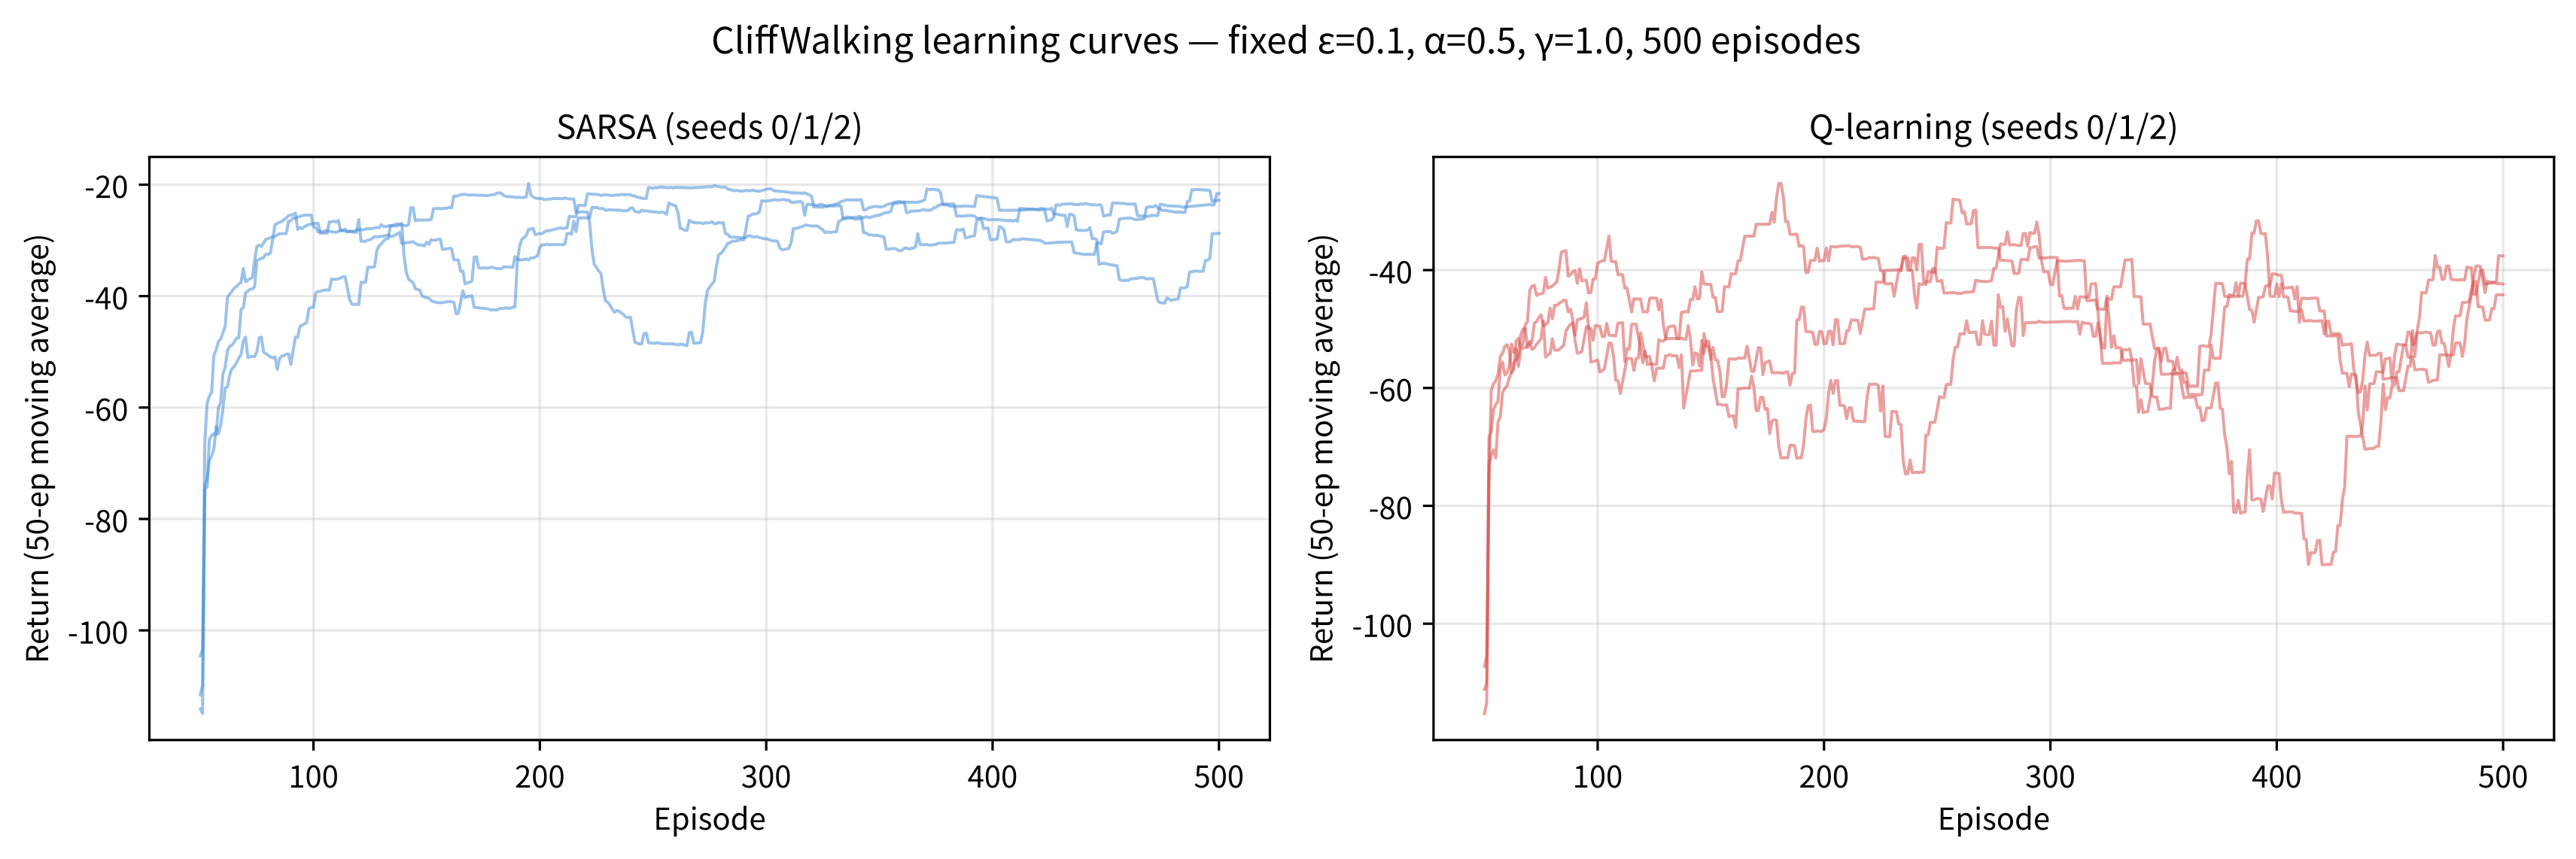
\includegraphics[width=\linewidth]{ch08_1_seeds_curves.png}
      \vskip0.3em
      {\footnotesize CliffWalking 학습 곡선(50 에피소드 이동평균).
      시드 0/1/2를 얇은 선으로 겹침 --- 시드마다 곡선이 \textbf{달라야
      정상}. 이 실험에서는 격차가 작았으나 \textbf{우연}일 수 있음.}
    \end{column}
    \begin{column}{0.5\textwidth}
      \begin{itemize}
        \item CliffWalking 시드 간 편차가 작았던 것은 \textbf{우연}일 수
          있고, 미리 아는 방법은 없다.
        \item 확률적 전이 환경(FrozenLake, 실습 §6): 같은 코드·파라미터를
          시드만 바꿔도 \textbf{같은 알고리즘의} greedy 평가가
          \textbf{0.045 / 0.090 / 0.125로 2.8배} 벌어짐.
        \item 시드 편차의 크기는 환경(확률 전이 여부, 상태 공간, 학습
          예산)에 달려 \textbf{실행하지 않고 알 수 없다}.
      \end{itemize}
      \vskip0.4em
      \kq{시드별 표는 형식적 서류가 아니라 ``결론의 신뢰도를 확인할
      수 있는 유일한 수단''.}
    \end{column}
  \end{columns}
\end{frame}

\begin{frame}{$\varepsilon$ 감쇠 스케줄도 하이퍼파라미터다}
  \begin{itemize}
    \item Ch\,6.3: $\varepsilon$를 내내 고정하면 ``탐험이 줄면서 배움이
      뎀프닝된다''. 프로젝트에서는 보통 \textbf{초반 높은 $\varepsilon$로
      넓게 방문 $\to$ 서서히 감쇠}.
    \item ``이 스케줄이 결과를 바꾸는가''는 \textbf{실험하지 않으면 답이
      없다} --- 실습: 스케줄 하나만 500 에피소드 1.0$\to$0.01 선형 감쇠로,
      \textbf{같은 파라미터·같은 시드}로 재실행.
    \item 결과: greedy 평가(SARSA $-17/-17/-17$, Q-learning
      $-13/-13/-13$)가 \textbf{한 치도 달라지지 않았다}.
  \end{itemize}
  \vskip0.5em
  \begin{block}{부정적 결과(negative result)도 결과다}
    ``이 환경·이 학습 예산에서 스케줄 선택이 성능에 민감하지 않다''는
    관찰도 보고서에 적어야 한다.
  \end{block}
  \vskip0.5em
  \begin{itemize}
    \item (a) \textbf{두 알고리즘 모두에게 동일한 스케줄} --- 한쪽에만 감쇠
      쓰면 ``감쇠의 효과''와 ``알고리즘의 차이''가 뒤섞임.
    \item (b) 다른 환경·예산에서 스케줄이 차이를 만들면 그 차이는
      \textbf{수식적 정당화}의 일부가 되어야 한다.
  \end{itemize}
\end{frame}

\begin{frame}[fragile]{선형 $\varepsilon$ 감쇠 스케줄 (핵심 코드)}
\begin{lstlisting}
def make_epsilon_schedule(n_episodes, eps_start=1.0, eps_end=0.01):
    def eps_fn(episode):  # 선형 감쇠
        return max(eps_end,
                   eps_start + (eps_end - eps_start) * episode
                   / n_episodes)
    return eps_fn
\end{lstlisting}
  \vskip0.4em
  \begin{itemize}
    \item $t=0$에서 $\varepsilon=1.0$(전부 탐험) $\to$ $t=$\texttt{n\_episodes}에서
      $0.01$로 선형 하강, \texttt{max}가 하한을 보장.
    \item 이 함수를 \textbf{두 알고리즘 모두}에 똑같이 전달하는 것이
      ``한 요인만 바꾸는'' 비교 실험의 원칙.
  \end{itemize}
\end{frame}

\begin{frame}{전체 그림: 4주 파이프라인}
  \begin{columns}[T]
    \begin{column}{0.6\textwidth}
      \centering
      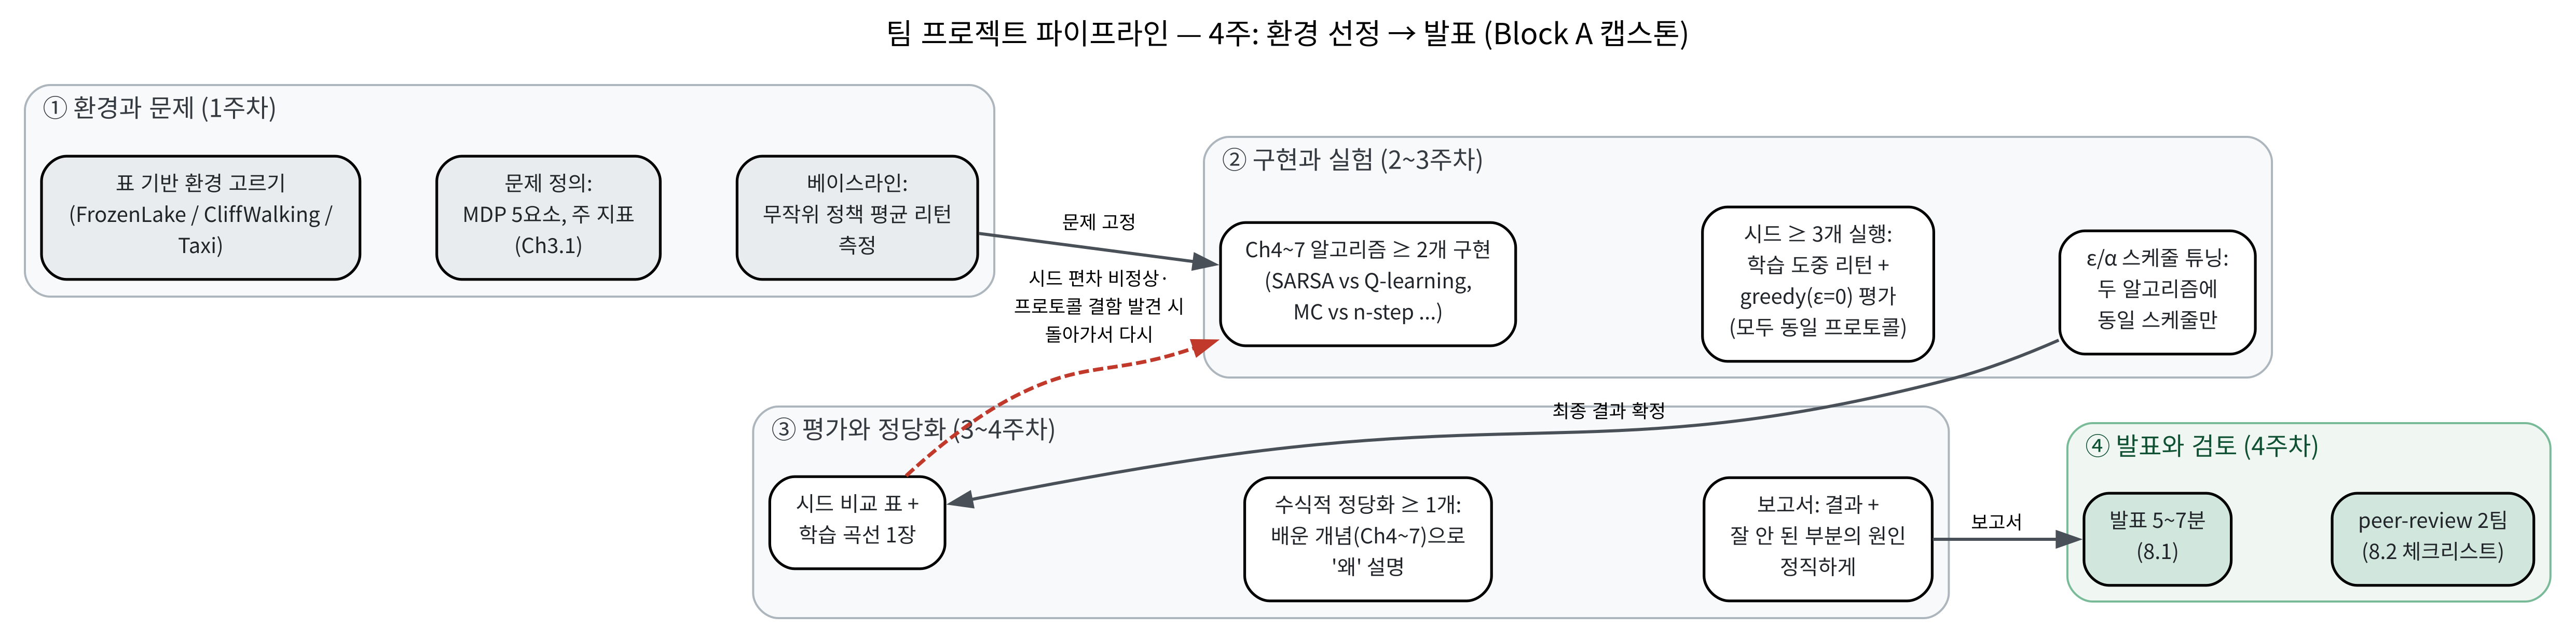
\includegraphics[width=\linewidth]{ch08_1_rl_pipeline.png}
      \vskip0.3em
      {\footnotesize 환경·문제 정의(1주) $\to$ 알고리즘 $\geq$2개 구현·
      시드 $\geq$3·학습 곡선(2$\sim$3주) $\to$ 수식적 정당화·보고서
      (3$\sim$4주) $\to$ 발표·peer-review(4주).}
    \end{column}
    \begin{column}{0.38\textwidth}
      \begin{itemize}
        \item 흐름: \textbf{환경 $\to$ 구현·비교 $\to$ 평가·정당화 $\to$
          발표}.
        \item \kq{붉은 점선(평가 $\to$ 구현·비교)이 핵심} --- 시드 간
          편차가 비정상적으로 크거나 평가 프로토콜 결함이 발견되면
          \textbf{돌아가서 다시}.
        \item ``한 번 지나가면 돌아올 수 없는'' 것은 \textbf{최종 발표
         뿐} --- 그 외 모든 단계는 되돌아갈 수 있다.
      \end{itemize}
    \end{column}
  \end{columns}
\end{frame}

\begin{frame}{일정과 마일스톤 M1$\sim$M4 (4주, 각 주 = 수업 3회)}
  \scriptsize
  \begin{tabular}{@{}clp{0.48\textwidth}p{0.24\textwidth}@{}}
    \toprule
    주 & 마일스톤 & 해야 할 일 & 제출물 \\
    \midrule
    1 & \textbf{M1} & 환경 후보 2$\sim$3개 조사(상태 수·보상 구조·확률 전이
      여부), 팀 회의, \textbf{문제 정의 문서} (어떤 MDP인지·어떤 지표
      쓸지·베이스라인(무작위 정책) 리턴) & 문제 정의 +
      환경 선택(1p) \\
    2 & \textbf{M2} & Ch\,6.3/7.3 코드에서 두 알고리즘 구현,
      \textbf{베이스라인 리턴 측정}, 시드 3개 중 1개에서 엔드투엔드
      동작 확인 & 중간코드 리뷰
      (코드 + 베이스라인 숫자 1줄) \\
    3 & \textbf{M3} & 나머지 시드 실행, $\varepsilon$/$\alpha$ 튜닝
      (모두 동일 프로토콜), \textbf{greedy 평가($\varepsilon=0$)},
      시드 비교 표 도출 & 학습 곡선 1장 +
      시드 비교 표 \\
    4 & \textbf{M4} & 수식적 정당화, 보고서·슬라이드 완성,
      \textbf{발표(5$\sim$7분)}, \textbf{peer-review 2팀} & 보고서 +
      발표 + 리뷰 2건 \\
    \bottomrule
  \end{tabular}
  \vskip0.8em
  {\footnotesize M1·M2는 팀 전체가 \textbf{모여 함께} 결정하는 것.}
\end{frame}

\begin{frame}{왜 마일스톤이 이 모양인가}
  \begin{columns}[T]
    \begin{column}{0.5\textwidth}
      \textbf{M2: 베이스라인 숫자 1줄}
      \begin{itemize}
        \item 이 숫자를 보고야 비로소 \textbf{``배운 정책이 무작위보다
          나은가''}를 판정.
        \item 절벽 예제: 무작위 정책은 500스텝 상한까지 돌아다니며
          절벽을 반복 타격 $\to$ 평균 리턴 \textbf{$-5{,}010$}
          (실측 100 에피소드).
        \item 이 제로점 덕분에 ``greedy 평가 $-17$''이 의미 있는
          숫자인지 바로 확인.
      \end{itemize}
    \end{column}
    \begin{column}{0.5\textwidth}
      \textbf{M3: 시드 비교 표}
      \begin{itemize}
        \item ``greedy 리턴 $-13$'' 한 줄만 내면 \textbf{시드 1개에서
          우연인지, 시드 3개에서 일관된지 검증 불가}.
        \item 표가 있어야 §비교 프로토콜을 \textbf{실제로 지켰는지가
          제출물에서 바로} 드러남.
      \end{itemize}
    \end{column}
  \end{columns}
  \vskip0.6em
  \begin{block}{공통 원리}
    제출물이 ``결과 1줄''이 아니라 ``결과 + 그 결과를 얻은 절차의 흔적''
    일 때, 채점(과 8.2의 리뷰)이 같은 언어로 작동한다.
  \end{block}
\end{frame}

\begin{frame}{손으로 한 번: ``수식적 정당화''의 좋은/나쁜 예}
  {\footnotesize 설정: 어떤 팀이 CliffWalking에서 ``Q-learning이 SARSA보다
  최종 평가 점수가 더 높았다 ($-13$ vs $-17$)''라는 결과를 얻었다.}
  \vskip0.5em
  \begin{alertblock}{나쁜 설명}
    ``Q-learning이 SARSA보다 점수가 더 높았다. Q-learning이 더 좋은
    알고리즘인 것 같다.''
  \end{alertblock}
  \vskip0.3em
  \begin{block}{좋은 설명 (요약)}
    학습 도중(탐험 포함)은 SARSA가 더 높았다 ($-31$ vs $-53$) --- Q-learning은
    \textbf{목표 정책(항상 최선)의 가치를 배우는 off-policy} 방법이라 절벽
    옆 최단 경로를 학습했고, 그 경로는 탐험 실수 한 번이 $-100$으로
    이어진다. SARSA는 \textbf{실제 행동 방식(탐험 포함)까지 감안하는
    on-policy}라 안전한 경로를 선호. 탐험 없이 평가하면 Q-learning 경로가
    더 짧아 $-13$ vs $-17$이지만, 이건 ``더 좋은 알고리즘''이 아니라
    \textbf{``두 알고리즘이 애초에 다른 질문에 답하고 있다''}.
  \end{block}
  \vskip0.4em
  \kq{같은 숫자를 말해도, 좋은 설명은 숫자 뒤의 \textbf{알고리즘의
  설계 차이}를 짚어낸다 --- 이것이 ``수식적 정당화''의 실제 의미.}
\end{frame}

\begin{frame}{보고서 구조 (M4): 4$\sim$6페이지, 6절}
  \small
  \begin{tabular}{@{}cp{0.68\textwidth}@{}}
    \toprule
    절 & 내용 \\
    \midrule
    1. 문제 정의 (0.5p) & MDP 5요소(Ch\,3.1): 상태·행동·전이·보상·할인율,
      \textbf{주 지표}(greedy 평가 평균 리턴), \textbf{베이스라인}(무작위
      정책 리턴) \\
    2. 알고리즘 선택과 이유 (1p) & 후보 $\geq 2$개, \textbf{왜 이
      알고리즘을 이 환경에} 골랐는가(보상 구조·상태 수와 연결),
      하이퍼파라미터($\alpha,\gamma,\varepsilon$ 스케줄)와 선택 근거 \\
    3. 실험 프로토콜 (1p) & 시드 목록, 학습 에피소드 수,
      \textbf{평가 프로토콜($\varepsilon=0$, 에피소드 수, 모든 알고리즘
      동일) 명시} --- 없으면 8.2 체크리스트에서 바로 감점 \\
    4. 결과 (1p) & 시드 비교 표, 학습 곡선 1장(여러 시드를 한 그림에
      얇은 선으로), greedy 정책 경로 시각화 \\
    5. 수식적 정당화 (1p) & Ch\,2$\sim$7 개념 $\geq 1$개로 ``왜 이
      결과'' --- §손으로 한 번의 좋은 예 문체 \\
    6. 잘 안 된 부분과 원인 진단 (0.5p) & \textbf{필수}. 없었으면
      ``무엇을 시도했다가 안 됐는가''를 씀 --- ``모두 잘 됐습니다''
      보고서는 이 절이 비어 있다는 뜻 \\
    \bottomrule
  \end{tabular}
  \vskip0.6em
  {\footnotesize 발표 슬라이드 = 보고서의 각 절 제목 --- 발표는 보고서의
  요약.}
\end{frame}

\begin{frame}{채점 기준 (rubric): 정직성이 절반}
  \small
  \begin{tabular}{@{}lp{0.08\textwidth}p{0.62\textwidth}@{}}
    \toprule
    항목 & 비중 & 좋은 답 \\
    \midrule
    문제 정의와 환경 & 15\% & MDP 5요소·지표·베이스라인이 명확하고,
      선택이 Ch\,4$\sim$7 개념 검증 목적에 근거 \\
    방법론 적절성 & 20\% & 환경 특성에 맞는 알고리즘·파라미터 선택,
      근거가 Ch\,4$\sim$7 개념으로 설명 \\
    \textbf{실험 프로토콜의 정직성} & \textbf{25\%} & 시드 $\geq 3$,
      동일 평가 프로토콜, 베이스라인, $\varepsilon$ 스케줄이 보고서에서
      추적 가능할 만큼 명시 \\
    수식적 정당화 & 20\% & 배운 개념 $\geq 1$개로 ``왜''를 설명했고,
      관측한 숫자와 일치 \\
    \textbf{결과의 정직성과 반성} & \textbf{20\%} & 불안정했던 시드·구간을
      숨기지 않고, 원인을 Ch\,4$\sim$7 개념으로 진단 \\
    \bottomrule
  \end{tabular}
  \vskip0.7em
  \begin{block}{우선순위}
    greedy가 $-13$이어도 프로토콜이 정직하고 정당화가 타당하면 고득점.
    $-13$이어도 \textbf{시드가 1개였다면} ``실험 프로토콜의 정직성''에서
    큰 감점 --- 8.2에서 다른 팀을 리뷰할 때도 정확히 이 순서.
  \end{block}
\end{frame}

\begin{frame}{자주 하는 실수 5가지 (1/2)}
  \begin{enumerate}
    \item \textbf{시드 1개 실험으로 결론} --- CliffWalking에서 편차가 작았
      = 이 환경의 성질이지 \textbf{보장}이 아님. FrozenLake(확률 전이)는
      시드만 바꿔도 greedy 평가가 0.045/0.090/0.125로 2.8배. 리뷰 질문:
      ``시드를 몇 개로 확인했나요? 시드 간 greedy 평가의 표준편차가
      알고리즘 간 차이보다 큰가요?''
    \item \textbf{평가 시에도 $\varepsilon$ 켜둔 채 비교} --- ``배운 정책의
      성능''이 아니라 ``탐험 10\%가 섞인 행동의 성능'' 측정. 게다가
      \textbf{비대칭적} --- 탐험이 섞이면 SARSA ``안전 경로''의 우위가
      상대적으로 줄어듦.
  \end{enumerate}
  \vskip0.6em
  {\footnotesize 각각이 Ch\,2$\sim$7의 어떤 원칙을 깨는지 짚어두면
  8.2에서 ``반박 가능한 질문''으로 바로 바뀐다.}
\end{frame}

\begin{frame}{자주 하는 실수 5가지 (2/2)}
  \begin{enumerate}
    \setcounter{enumi}{2}
    \item \textbf{알고리즘마다 다른 $\varepsilon$ 스케줄} --- ``Q-learning
      고정 0.1, SARSA 감쇠''는 알고리즘 차이에 스케줄 효과가 뒤섞임
      (\textbf{한 요인만 바꾸는} 것이 비교 실험의 원칙).
    \item \textbf{베이스라인 없이 ``잘 배웠다'' 발표} --- 절벽 환경에서
      무작위 정책 평균 리턴은 $-5{,}000$ 수준(실측 $-5{,}010$).
      \textbf{측정 없이 말하는 것}과 ``측정해서 아는 것''이 보고서
      수준을 가른다.
    \item \textbf{``곡선이 잘 올라갔으니 성공''으로 진단 건너뛰기} ---
      잘 올라가도 \textbf{시드 간 편차}와 \textbf{평가 프로토콜}을
      확인해야 ``성공'' --- 없다면 ``무엇을 시도했다가 안 됐는가''가
      필수 절의 존재 이유.
  \end{enumerate}
\end{frame}

\begin{frame}{발표: 5$\sim$7분, 마지막 1분이 가장 평가받는다}
  \begin{itemize}
    \item 구조: 문제 정의(1분) $\to$ 알고리즘과 이유(2분) $\to$
      학습 곡선/최종 정책 비교 + 수식적 정당화(2$\sim$3분) $\to$
      \textbf{잘 안 됐던 부분과 원인 진단(1분)}.
    \item ``최종 greedy 리턴 $-13$이었다''보다 \textbf{``왜 이
      알고리즘을 이 환경에 골랐고, 왜 이 결과가 나왔는지''}를
      설명하는 쪽에 더 높은 점수.
  \end{itemize}
  \vskip0.6em
  \begin{block}{``모든 것이 잘 됐다''는 발표는 스스로 감점}
    예: ``Q-learning greedy $-13$, SARSA $-17$ --- 4스텝 차이가 시드 3개에서
    재현됐고, 6.3절 on/off-policy 차이(절벽 옆 최단 vs 안전 경로)로
    설명된다. 다만 FrozenLake 2차 실험에서는 MC greedy 0.045/0.090/0.125,
    SARSA 0.245/0.525/0.730으로 시드마다 크게 벌어져, ``MC가 못
    한다''는 결론은 내리지 못했다 --- 시드 5개로 재확인을 계획한다.''
    --- \textbf{실패에 가까운 실험까지 배운 개념으로 해석한} 증거.
  \end{block}
  \vskip0.5em
  {\footnotesize Block B Ch\,16.1(신경망 RL 캡스톤)도 동일한 구조 ---
  이 습관(시드, 평가 분리, 반박 가능한 질문)이 학기 말까지 이어진다.}
\end{frame}

\begin{frame}{실습: 미니 프로젝트를 한 흐름으로 (6단계)}
  \begin{columns}[T]
    \begin{column}{0.56\textwidth}
      \small
      \begin{enumerate}
        \item \textbf{CliffWalking-v1} --- 4$\times$12 격자, 절벽 $-100$
          (6.3절과 같은 \texttt{gym.make("CliffWalking-v1")}).
        \item \textbf{SARSA와 Q-learning 구현} --- Ch\,6.3의 두 갱신 규칙
          그대로.
        \item \textbf{고정 $\varepsilon=0.1$, 500 에피소드, 시드 0/1/2} ---
          학습 도중 리턴 vs greedy 평가 비교.
        \item \textbf{greedy 정책 경로 시각화} --- 절벽 옆 최단(13스텝)
          vs 안전(17스텝)이 눈에 보도록.
        \item \textbf{$\varepsilon$ 감쇠(1.0$\to$0.01) 재실행} --- 같은
          파라미터·시드로 스케줄 하나만 바꿔 greedy 평가 변화 확인
          (변하지 않음 --- 부정적 결과도 결과).
        \item \textbf{FrozenLake-v1: MC 제어(첫방문, Ch\,5.3) vs SARSA} ---
          1000 에피소드, 시드 3개. 확률 전이 환경에서는 같은 알고리즘의
          greedy 평가도 시드마다 크게 벌어짐 (MC: 0.045/0.090/0.125).
      \end{enumerate}
    \end{column}
    \begin{column}{0.4\textwidth}
      \centering
      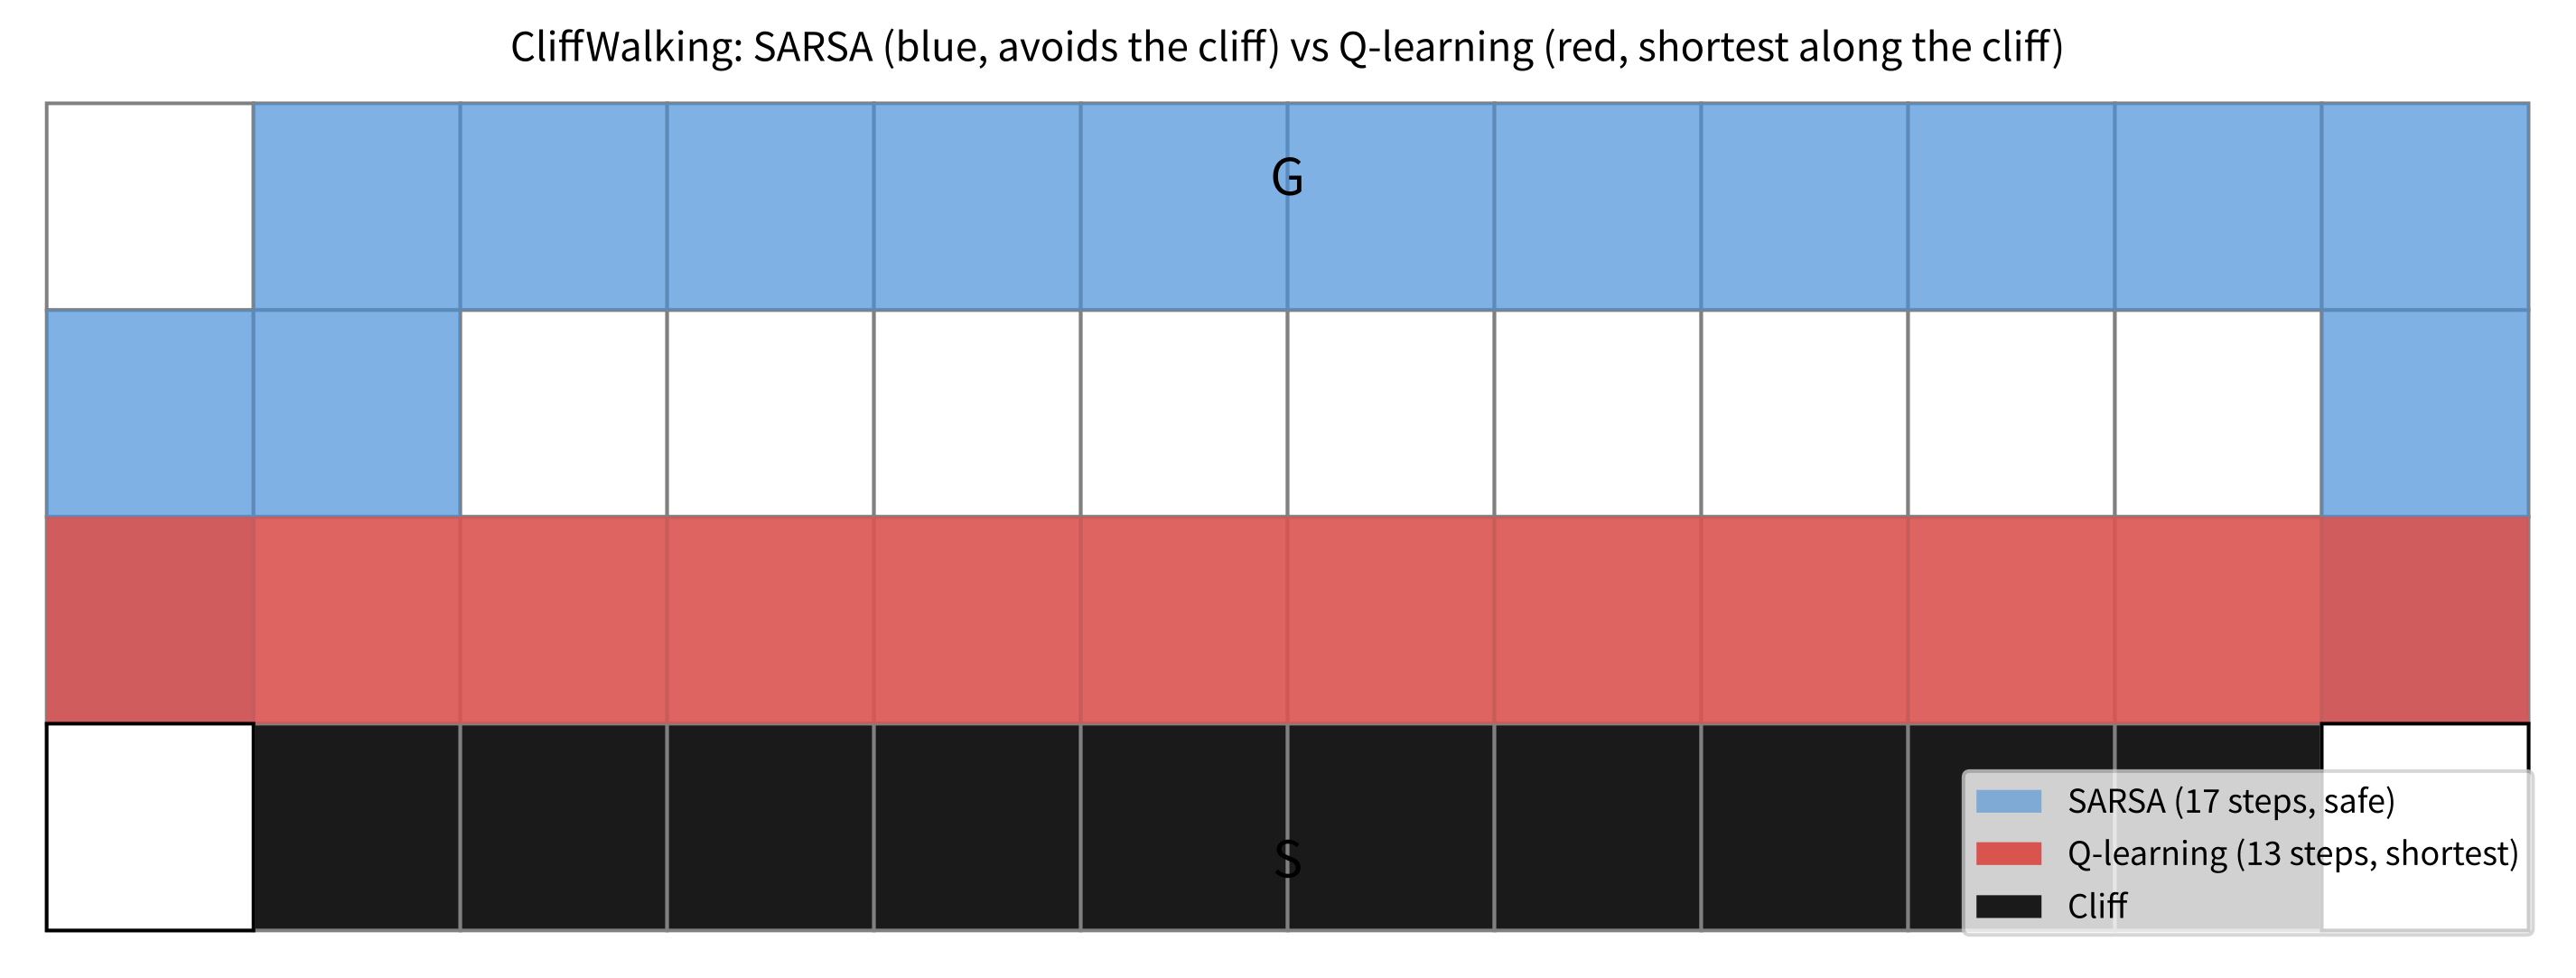
\includegraphics[width=\linewidth]{ch08_1_cliff_paths.png}
      \vskip0.3em
      {\footnotesize greedy 정책 경로 --- SARSA(파랑)는 절벽에서
      떨어진 위쪽 17스텝, Q-learning(빨강)은 절벽 바로 옆 13스텝.
      6.3절 on/off-policy 차이를 한 장에.}
    \end{column}
  \end{columns}
  \vskip0.4em
  \begin{block}{세 가지 언어}
    이 6단계 = 보고서 6절 = 8.2 체크리스트 4항목. \textbf{코드, 보고서,
    리뷰로 같은 절차를 말할 수 있어야} 프로젝트가 끝난 것.
  \end{block}
\end{frame}

\begin{frame}{확인 문제 (1/2): 절차가 개념을 요구할 때}
  \small
  \begin{block}{Q1. 시드 2 \textbf{하나}만 돌려 Q $-13$, SARSA $-17$을 얻고
  ``Q-learning이 더 좋다''고 결론}
  \begin{itemize}
    \item 시드 1개의 greedy 평가는 ``무작위성 한 번''의 결과 --- 시드 2가
      \textbf{우연히} 편차가 작은 시드였을 수 있음.
    \item 재실행: ``SARSA $-17/-17/-17$, Q $-13/-13/-13$''처럼 \textbf{시드별
      숫자가 일관}되면, 결론은 ``greedy 평가에서 Q-learning이 4스텝 꾸준히
      앞선다 --- 6.3절 on/off-policy 설계 차이''로 \textbf{격상}.
    \item 단, ``이 환경에서 편차가 작았음''은 환경의 보장이 아님
      (FrozenLake)임을 함께 적어야 \textbf{정직한 보고}.
    \item 또한 이 비교는 ``\textbf{탐욕적 실행} 시 어느 정책이 나은가''의
      답이지 ``더 좋은 알고리즘''의 답이 아님.
  \end{itemize}
  \end{block}
  \vskip0.4em
  \begin{block}{Q2. ``$\varepsilon$ 스케줄을 종료 시점에 0.1로, 최종 평가는
  탐험 없이 했다''는 프로토콜 문장의 결함}
  \begin{itemize}
    \item $\varepsilon=0.1$이면 매 스텝 10\% 확률로 무작위 행동이
      들어감 $\to$ ``탐험 없이''와 \textbf{모순}.
    \item 고쳐 쓰기: (a) 학습 스케줄: 1.0$\to$0.01 선형 감쇠,
      (b) 최종 평가: $\varepsilon=0$ (greedy), 200 에피소드,
      모든 알고리즘·시드에 \textbf{동일} --- \textbf{학습 스케줄과
      평가 프로토콜을 따로} 명시.
  \end{itemize}
  \end{block}
\end{frame}

\begin{frame}{확인 문제 (2/2): 두 층의 불확실성, 좋은 정당화}
  \small
  \begin{block}{Q3. ``MC 분산이 크므로 greedy 평가 에피소드를 10{,}000개로
  늘리자'' --- 학습/평가 에피소드 수는 각각 어떤 불확실성을 줄여주나}
  \begin{itemize}
    \item \textbf{평가} 에피소드 = \textbf{고정된} 정책의 성능 측정
      \textbf{오차}만 줄임 --- 나쁜 정책 10{,}000번 = 나쁜 정책의
      정확한 평균.
    \item \textbf{시드} = \textbf{어떤 정책이 학습됐는가}의 학습 과정
      무작위성 --- FrozenLake처럼 0.045/0.090/0.125(2.8배) 흩어지는 것은
      측정 오차가 아니라 \textbf{학습 결과의 차이}, 평가 에피소드로
      사라지지 않음. (ML1 8.1: ``어떤 모델이 나왔는가'' vs ``재는
      오차'')
  \end{itemize}
  \end{block}
  \vskip0.4em
  \begin{block}{Q4. ``$\varepsilon$-greedy라 학습이 진행되면 탐험 비중이 줄고
  성과가 좋아졌다'' --- 좋은 예인가}
  \begin{itemize}
    \item \textbf{나쁜 예}에 가깝다 --- 장치를 기계적으로 서술할 뿐,
      6.3절 개념 + \textbf{실측 숫자의 일치}가 없음.
    \item 좋은 예는 \textbf{정의($\varepsilon$-greedy) + 환경 구조($-100$)
      + 실측 숫자의 삼박자}: 고정 $\varepsilon=0.1$에서 Q 학습중 리턴
      (시드 평균 $\approx -50$)이 SARSA($\approx -26$)의 2배로 나쁘다
      --- $\varepsilon=0.1$이면 절벽 옆 13스텝 경로에서 에피소드당
      $1-0.9^{13}\approx 0.73$ 확률로 무작위 행동이 1회 이상, 그것이
      ``아래''면 $-100$ $\to$ 학습중 손실의 대부분이 절벽 사고.
      (참고: $1-0.9^{13}\approx 0.73$, $1-0.99^{13}\approx 0.12$ ---
      절벽 사고 기대 빈도 \textbf{예측}은 성립하지만, 실제로 학습중
      리턴이 그만큼 개선되지는 않음: §$\varepsilon$ 감쇠의 부정적 결과.)
  \end{itemize}
  \end{block}
\end{frame}

\begin{frame}{자주 묻는 질문 (8.1)}
  \scriptsize
  \begin{tabular}{@{}p{0.3\textwidth}p{0.66\textwidth}@{}}
    \toprule
    질문 & 핵심 답 \\
    \midrule
    두 알고리즘 성능이 거의 같으면 & ``비슷하다''는 것 자체가 관찰 ---
      학습중/학습후를 \textbf{나눠} 보면 겉보기엔 비슷해도 다른
      트레이드오프라는 것을 발견할 수 있음 \\
    매번 결과가 달라 비교가 안 되면 & $\varepsilon$ 여러 개로 반복 실행한
      평균(과 가능하면 분산) 비교가 \textbf{표준적 방법} \\
    시드 몇 개가 정석인가 & 실행 비용 vs 결론 안정성의 절충 --- 표 기반
      환경은 시드당 몇 초$\sim$분 $\to$ \textbf{3$\sim$5개 현실적 하한},
      10개면 더 단단. 표준편차 1개 안에 겹치면 정직한 결론 =
      ``유의미한 차이 관측 불가'' \\
    코드를 처음부터 써야 하나 & 강의 코드 재용이 \textbf{전제} ---
      (a) 재사용한 부분(Ch\,6.3 갱신 규칙)과 (b) 팀이 수정·추가한
      부분(환경 인터페이스, 시드 처리, 평가 프로토콜)을 \textbf{구분}
    \midrule
    시간이 부족해 시드를 5$\to$3개로 줄였으면 & 성공 기준은 ``깨끗한
      숫자''가 아니라 \textbf{``정직한 절차''} --- ``시간 부족으로
      3시드로만 확인, SARSA 시드 간 편차가 커서 5시드 재확인 권장''을
      ``잘 안 된 부분''에 쓰는 것이 감추는 것보다 항상 낫다 \\
    \bottomrule
  \end{tabular}
\end{frame}

\section{8.2 Peer-Review}

\begin{frame}{왜 Peer-Review인가: 이번 주에는 네가 심사위원이다}
  \begin{itemize}
    \item 4주 파이프라인에서 4주째는 \textbf{역전} --- 발표팀이었던 각
      팀이 \textbf{다른 두 팀의 발표를 심사}하고 리뷰 \textbf{2통}을 작성.
    \item 채점 대상은 리뷰의 \emph{양}이 아니라 \emph{질}: ``4항목을
      다 썼는가''가 아니라 \textbf{``그 질문이 반박 가능한 질문인가''}.
  \end{itemize}
  \vskip0.6em
  \begin{block}{근거 (ML1 8.2에서 그대로 이어받음)}
    \begin{itemize}
      \item Popper의 \textbf{반증주의}: 한 주장은 ``그것이 틀렸음을
        보여주는 관측이 상상이 가능한가''로 판별.
      \item Amgen 재현 실험(2011): 53편의 'landmark' 논문 중 \textbf{6편
        만} 재현. \kq{좋은 결과는 스스로를 증명하지 못하고, 결과가
        남이 재현·반박할 수 있도록 만들어졌는지가 기준.}
      \item 강화학습에서는 이 위험이 \textbf{더 높음} --- 결과를 내는
        \textbf{과정 자체}가 무작위(시드, 탐험)라 ``우연히 좋은''
        확률이 학습모델보다 훨씬 큼.
    \end{itemize}
  \end{block}
\end{frame}

\begin{frame}{이번 주는 어떻게 진행되는가}
  \small
  \begin{tabular}{@{}clp{0.6\textwidth}@{}}
    \toprule
    순서 & 내용 & 시간 배분 \\
    \midrule
    1 & 다른 두 팀의 발표 청취(팀당 5$\sim$7분, 8.1 형식 그대로) +
      보고서·슬라이드 열람 & 약 30분 \\
    2 & \textbf{작성 리뷰 2통} --- 팀당 체크리스트 4항목 + \textbf{반박
      가능한 질문 1개 이상}(개념의 장·절 명시) & 발표 직후(각 10분) \\
    3 & 질의·토론 --- 리뷰어가 쓴 질문에 발표팀이 그 자리에서 답변 &
      나머지 시간 \\
    \bottomrule
  \end{tabular}
  \vskip0.8em
  \begin{itemize}
    \item 핵심은 2번의 \textbf{작성 리뷰}. 3번 토론은 ``발표팀이 그 질문에
      \textbf{실제로} 답할 수 있는가''를 가르는 자리.
    \item \kb{3점 질문} = 답하려면 \textbf{새로운 계산·실험}(시드 재실행,
      $\varepsilon=0$ 재평가, $\alpha$ 민감성 등)을 꺼내야 하는 질문.
      ``네, 알겠습니다''로 넘어가는 질문은 2점에 머물러.
    \item 8.1에서 ``수식적 정당화''가 발표팀의 \emph{의무}였다면, 이번 주
      그 정당화가 \emph{타당한지}를 리뷰어가 \emph{심사}.
  \end{itemize}
\end{frame}

\begin{frame}{Peer-Review 체크리스트 4항목}
  \small
  \begin{tabular}{@{}lp{0.62\textwidth}@{}}
    \toprule
    항목 & 확인할 것 \\
    \midrule
    1. 환경 설명 & 상태·행동·보상이 명확히 정의됐는가 --- ``CliffWalking을
      썼다'' 한 줄 + \textbf{주 지표}(학습중 리턴? greedy 평가? 에피소드
      길이?) 없으면 뒤의 모든 숫자가 ``무엇의 평균''인지 모름.
      8.1의 학습중/학습후 \textbf{분리}가 이 항목의 핵심. \\
    2. 알고리즘 선택 & \textbf{이 환경의 어떤 특성}(상태 공간, 보상 구조,
      확률 전이)이 그 비교를 정당화하는가. FrozenLake(16$\times$4) vs
      Taxi(500$\times$6)의 n-step vs MC는 설계 난이도가 완전히 다르다.
      선택은 자유, \textbf{설명 가능한 연결}이 필요. \\
    3. 수식적 정당화 & 요구사항($\geq 1$개)은 형식, 이 항목은 \textbf{내용}:
      짚은 개념(Ch\,6.3 on/off-policy)이 \textbf{실측 숫자}
      (학습중 $-50$ vs $-32$, greedy $-13$ vs $-17$)와 일치하는가.
      숫자 없는 문장은 ``어디에나 붙을'' 설명. \\
    4. 결과의 정직성 & 시드 $\geq 3$, 시드별 숫자 표, \textbf{불안정했던
      시드·구간이 사라지지 않고} 들어갔는가. ``결과가 좋았나''가 아니라
      ``\textbf{정직한 절차}로 얻어졌나''. \\
    \bottomrule
  \end{tabular}
  \vskip0.6em
  {\footnotesize 4항목 = 8.1 rubric의 축 --- 리뷰어와 발표팀이 \textbf{같은
  기준표}를 공유해야 ``감점''과 ``좋은 지적''이 같은 언어.}
\end{frame}

\begin{frame}{채점 기준: ``채웠는가''가 아니라 ``구체적인가''}
  \scriptsize
  \begin{tabular}{@{}lp{0.3\textwidth}p{0.44\textwidth}@{}}
    \toprule
    리뷰 품질 & 특징 & 예시 (CliffWalking) \\
    \midrule
    \textbf{1점 — 감상평} & 구체적 지적 없음, 느낌만 & ``학습 곡선이
      꾸준히 올라가서 잘된 것 같습니다.'' \\
    \textbf{2점 — 일반 지적} & 문제를 제기하지만 \textbf{근거(개념) 약함},
      발표팀이 ``네''로 넘길 수 있음 & ``시드를 하나 더 돌려서
      확인해보는 게 좋을 것 같습니다.'' \\
    \textbf{3점 — 반박 가능한 질문} & \textbf{이 학기 개념(장·절) 명시} +
      \textbf{답이 나쁘면 결과가 흔들림} & ``최종 평가가 $\varepsilon=0$로
      했나요? $\varepsilon=0.1$으로 평가한 채로는 Q $-45$, SARSA $-21$로
      \textbf{결론이 뒤집힙니다}(Ch\,6.3 on/off-policy 경로 차이).'' \\
    \bottomrule
  \end{tabular}
  \vskip0.8em
  \begin{block}{1점$\to$3점의 공통 패턴}
    추상적 평가어(``잘됐다'', ``확인해보라'')를 (a) \textbf{구체적 관찰}
    + (b) \textbf{이 학기 개념(Ch\,NN)} + (c) \textbf{왜 문제인지
    (숫자)}로 교체하는 것.
  \end{block}
\end{frame}

\begin{frame}{손으로 한 번: 가상 발표 (팀 ``절벽우회'')}
  \begin{block}{발표 요약}
    ``CliffWalking에서 SARSA와 Q-learning을 비교했다. $\alpha=0.5$,
    $\gamma=1.0$, $\varepsilon=0.1$ 고정, 500 에피소드, \textbf{시드 0}으로
    학습했다. 학습 곡선이 꾸준히 올라가서 잘 됐다. 최종 평가(학습된 정책
    200 에피소드)에서 \textbf{SARSA $-21.3$, Q-learning $-45.3$}이라
    SARSA가 더 좋은 알고리즘이다. Ch\,6.3에서 SARSA가 절벽을 피하는 안전
    알고리즘이라 배웠으니 일치한다.'' --- 문제인 곳은 숫자가 아니라
    \textbf{프로토콜}.
  \end{block}
  \vskip0.5em
  \begin{itemize}
    \item \textbf{환경 설명} --- 환경은 명확(4$\times$12, 절벽 $-100$)
      하지만 \textbf{주 지표 모호}: ``200 에피소드''가 $\varepsilon=0$인지,
      학습 때 쓰던 0.1인지 문장에 없음 $\to$ 8.1이 \textbf{분리}를
      요구한 이유.
    \item \textbf{알고리즘 선택} --- SARSA vs Q-learning은 절벽 $-100$
      보상 구조에 가장 잘 맞는 비교 $\to$ \textbf{통과}.
  \end{itemize}
\end{frame}

\begin{frame}{가상 발표 리뷰: 정당화와 정직성}
  \begin{itemize}
    \item \textbf{수식적 정당화} --- Ch\,6.3을 \emph{인용}했지만 인용과
      관측이 \textbf{연결되어 있지 않아}: ``SARSA가 안전 알고리즘''은
      \emph{학습 도중} 성과에 관한 이야기인데, 발표 숫자는
      \emph{최종 평가} 비교. 게다가 그 평가가 $\varepsilon=0$이 아니라면
      Ch\,6.3의 설명은 \emph{그 상황}에 해당하지 않음 $\to$ 개념을
      끌고 와 숫자에 \textbf{끼워 맞춘 = 형식만 있는 정당화}.
    \item \textbf{결과의 정직성} --- 세 가지가 \textbf{사라져 있음}:
    \begin{itemize}
      \item (1) \textbf{시드 1개} --- 시드 1개의 ``최종 평가''는 학습
        과정의 우연 (8.1: SARSA 시드 2번 $-200$ 고착 사례).
      \item (2) \textbf{베이스라인(무작위) 부재} --- ``잘 배웠다''의
        기준점 자체.
      \item (3) \textbf{평가 $\varepsilon$ 미명시} --- §실습에서 이것이
        \textbf{결론의 방향}을 가름한 변수.
    \end{itemize}
  \end{itemize}
  \vskip0.5em
  \begin{block}{3점 질문 (이 발표를 향해)}
    ``최종 200 에피소드 평가는 $\varepsilon=0$로 했나요? 같은 학습 결과를
    $\varepsilon=0.1$로 평가하면 Q $-45.3$, SARSA $-21.3$으로
    \textbf{SARSA가 더 좋아 보이고}, 반대로 $\varepsilon=0$이면 Q $-13$,
    SARSA $-17$으로 \textbf{순위가 뒤집힙니다}(Ch\,6.3: 절벽 옆 경로는
    탐험 한 번이 $-100$). \textbf{두 프로토콜 모두 시드 3개로 재실행
    해주세요.}''
  \end{block}
  {\footnotesize 3점인 이유: 답하려면 \textbf{새 실험}($\varepsilon=0$
  재실행 + 시드 2개 추가)이 필요하고, 그 실험을 돌리면 결론이 흔들릴
  수 있음.}
\end{frame}

\begin{frame}{``우연히 좋은'' 패턴 5가지 (1/2)}
  {\footnotesize ML1에서 원천 = 테스트셋 유출·정확도의 함정·과적합.
  강화학습에는 \textbf{검증/테스트셋 자체가 없으니} 학습 과정의
  \textbf{무작위성}이 같은 역할. 8.1 실수 5가지의 \emph{리뷰어 눈} 버전.}
  \vskip0.4em
  \scriptsize
  \begin{tabular}{@{}p{0.16\textwidth}p{0.24\textwidth}p{0.26\textwidth}p{0.30\textwidth}@{}}
    \toprule
    패턴 & 겉보기 & 실제로는 & 반박 가능한 질문(근거) \\
    \midrule
    \textbf{1. 시드 1개 학습 곡선} & ``곡선이 잘 올라가네'' & 학습 과정의
      우연 --- $\varepsilon$-greedy + (FrozenLake 등) 전이 무작위성,
      같은 코드도 매번 다른 곡선 & ``시드 2개 더 돌리면 greedy 평가의
      표준편차가? 알고리즘 간 차이가 그 편차보다 큰가요?''(8.1 §비교
      프로토콜) \\
    \textbf{2. 평가 시에도 $\varepsilon$ 켜둔 채} & ``최종 정책의 성과다'' &
      ``탐험이 섞인 행동''의 성과 --- CliffWalking에서 탐험 혼입 시
      \textbf{Q만 급격히} 망가지고($-13\to-45$), SARSA는 거의 안
      흔들림($-17\to-21$) & ``최종 평가가 $\varepsilon=0$이었나요?
      $\varepsilon=0.1$로 하면 \textbf{순위가 뒤집힙니다}(Ch\,6.3 경로
      차이)''(§실습 2) \\
    \textbf{3. 알고리즘마다 다른 $\varepsilon$ 스케줄} & ``각자가 최적의
      설정으로'' & \textbf{한 요인만 바꾸는} 비교 실험 원칙 위반 ---
      알고리즘 차이와 스케줄 효과가 뒤섞임 & ``두 알고리즘에 \textbf{같은
      스케줄}을 적용했나요? 한쪽만 감쇠했다면 어떻게 분리했나요?''(8.1
      §자주 하는 실수) \\
    \bottomrule
  \end{tabular}
\end{frame}

\begin{frame}{``우연히 좋은'' 패턴 5가지 (2/2): 4·5}
  \scriptsize
  \begin{tabular}{@{}p{0.16\textwidth}p{0.24\textwidth}p{0.26\textwidth}p{0.30\textwidth}@{}}
    \toprule
    패턴 & 겉보기 & 실제로는 & 반박 가능한 질문(근거) \\
    \midrule
    \textbf{4. 하이퍼파라미터 ``적당히'' 하나} & ``$\alpha=0.5$로 학습'' &
      \textbf{민감성 미검증} --- Ch\,7.2 n 튜닝처럼 $\alpha$가 크면
      (0.5) Q값이 노이즈에 크게 흔들려 정책이 달라질 수 있음 &
      ``$\alpha$를 0.1로 줄이면 \textbf{결론이 변하나요}? 민감성을
      확인했나요?''(Ch\,7.2 튜닝) \\
    \textbf{5. 베이스라인 없이 ``잘 배웠다''} & ``$-13$이 나왔다'' &
      기준점 없이 ``나다''를 말할 수 없음 --- 무작위 정책 평균 리턴
      (약 $-5000$)을 재야 ``실제로 이득인가'' 판정 가능 & ``무작위
      정책의 평균 리턴은? 배운 정책이 그 대비 얼마나 \textbf{나은지
      측정}했나요?''(8.1 M2) \\
    \bottomrule
  \end{tabular}
  \vskip0.7em
  \begin{block}{패턴 2가 특히 RL \emph{특유}인 이유}
    \textbf{비대칭성} --- 탐험 혼입 시 두 알고리즘이 \emph{다른 방향의
    크기}로 망가지는 것. Ch\,6.3 on/off-policy 경로 차이를
    \textbf{정량적}으로 이해해야 짚어낼 수 있는, 이번 학기 개념이
    직접 작동하는 지점.
  \end{block}
\end{frame}

\begin{frame}{실습 (1/3): 발표팀 재현 + $\varepsilon=0$ 재평가}
  \begin{enumerate}
    \item \textbf{발표팀 재현} --- CliffWalking에서 SARSA·Q-learning,
      시드 0, $\alpha=0.5$, $\gamma=1.0$, $\varepsilon=0.1$ 고정,
      500 에피소드. \textbf{평가도 $\varepsilon=0.1$}으로 200 에피소드
      $\to$ SARSA $-21.3$ vs Q-learning $-45.3$ (발표팀 숫자 재현).
    \item \textbf{패턴 2 검증 --- 평가 $\varepsilon$을 0으로} --- 같은
      학습 결과를 $\varepsilon=0$(탐욕적)으로 200 에피소드 재평가
      $\to$ \textbf{Q-learning $-13$(13스텝) vs SARSA $-17$(17스텝):
      순위가 뒤집힌다.}
  \end{enumerate}
  \vskip0.5em
  \begin{block}{왜 Q-learning 쪽만 크게 망가지나 (손계산)}
    \begin{itemize}
      \item \textbf{Q-learning (13스텝)}: 절벽 \textbf{바로 위(2행)}를
        11스텝 이동 --- 스텝당 추락 확률 $0.1\times\tfrac14=0.025$
        $\to$ 12스텝 중 한 번이라도 $1-0.975^{12}\approx 0.26$.
        $\approx 0.74(-13)+0.26(-107)\approx -38$.
      \item \textbf{SARSA (17스텝)}: 0$\sim$1행 \textbf{위쪽 우회} ---
        추락하려면 \textbf{랜덤 두 번}(연이어 ``아래'') 필요, 스텝당
        $0.025^2$로 \textbf{2차적} $\to$ $\approx -20$ 부근.
    \end{itemize}
  \end{block}
\end{frame}

\begin{frame}{실습 (2/3): 비대칭의 기원 + 시드·베이스라인}
  \begin{itemize}
    \item 손계산(약 $-38$ / 약 $-20$)과 시뮬레이션($-45.3$ / $-21.3$)이
      \textbf{같은 크기·같은 순서}. Q 쪽 차이는 추락 시 깊이 분포 +
      랜덤 우회 스텝의 추가 비용.
    \item \kq{``절벽과 한 스텝'' 경로와 ``절벽과 두 스텝'' 경로는
      $\varepsilon$이 섞이는 순간 추락 확률이 \textbf{1차 vs 2차}로
      갈라서 성과 격차가 크게 벌어진다.}
  \end{itemize}
  \vskip0.5em
  \begin{enumerate}
    \setcounter{enumi}{2}
    \item \textbf{패턴 1 검증 --- 시드 2개 추가} --- 시드 1, 2로 같은
      프로토콜 재실행 $\to$ 시드별 greedy 표. (이번 실행에서는 3시드
      모두 $-13/-13/-13$, $-17/-17/-17$로 일관. 단, 8.1처럼 설정이
      조금만 달라지면 SARSA 시드 2번 $-200$ 고착도 --- ``시드 3개''가
      \textbf{형식이 아니라 정량적} 요구인 이유.)
    \item \textbf{패턴 5 검증 --- 베이스라인} --- 무작위 정책 500
      에피소드 $\to$ 평균 약 \textbf{$-5036$}(평균 486스텝, 절벽 반복
      추락). 배운 정책($-13/-17$)의 이득이 \textbf{측정된} 기준점
      위에서 확인.
    \item \textbf{리뷰 작성} --- 실습 숫자를 근거로 3점 리뷰를 템플릿으로
      완성.
  \end{enumerate}
\end{frame}

\begin{frame}{실습 (3/3): 평가 $\varepsilon$의 비대칭}
  \begin{columns}[T]
    \begin{column}{0.58\textwidth}
      \centering
      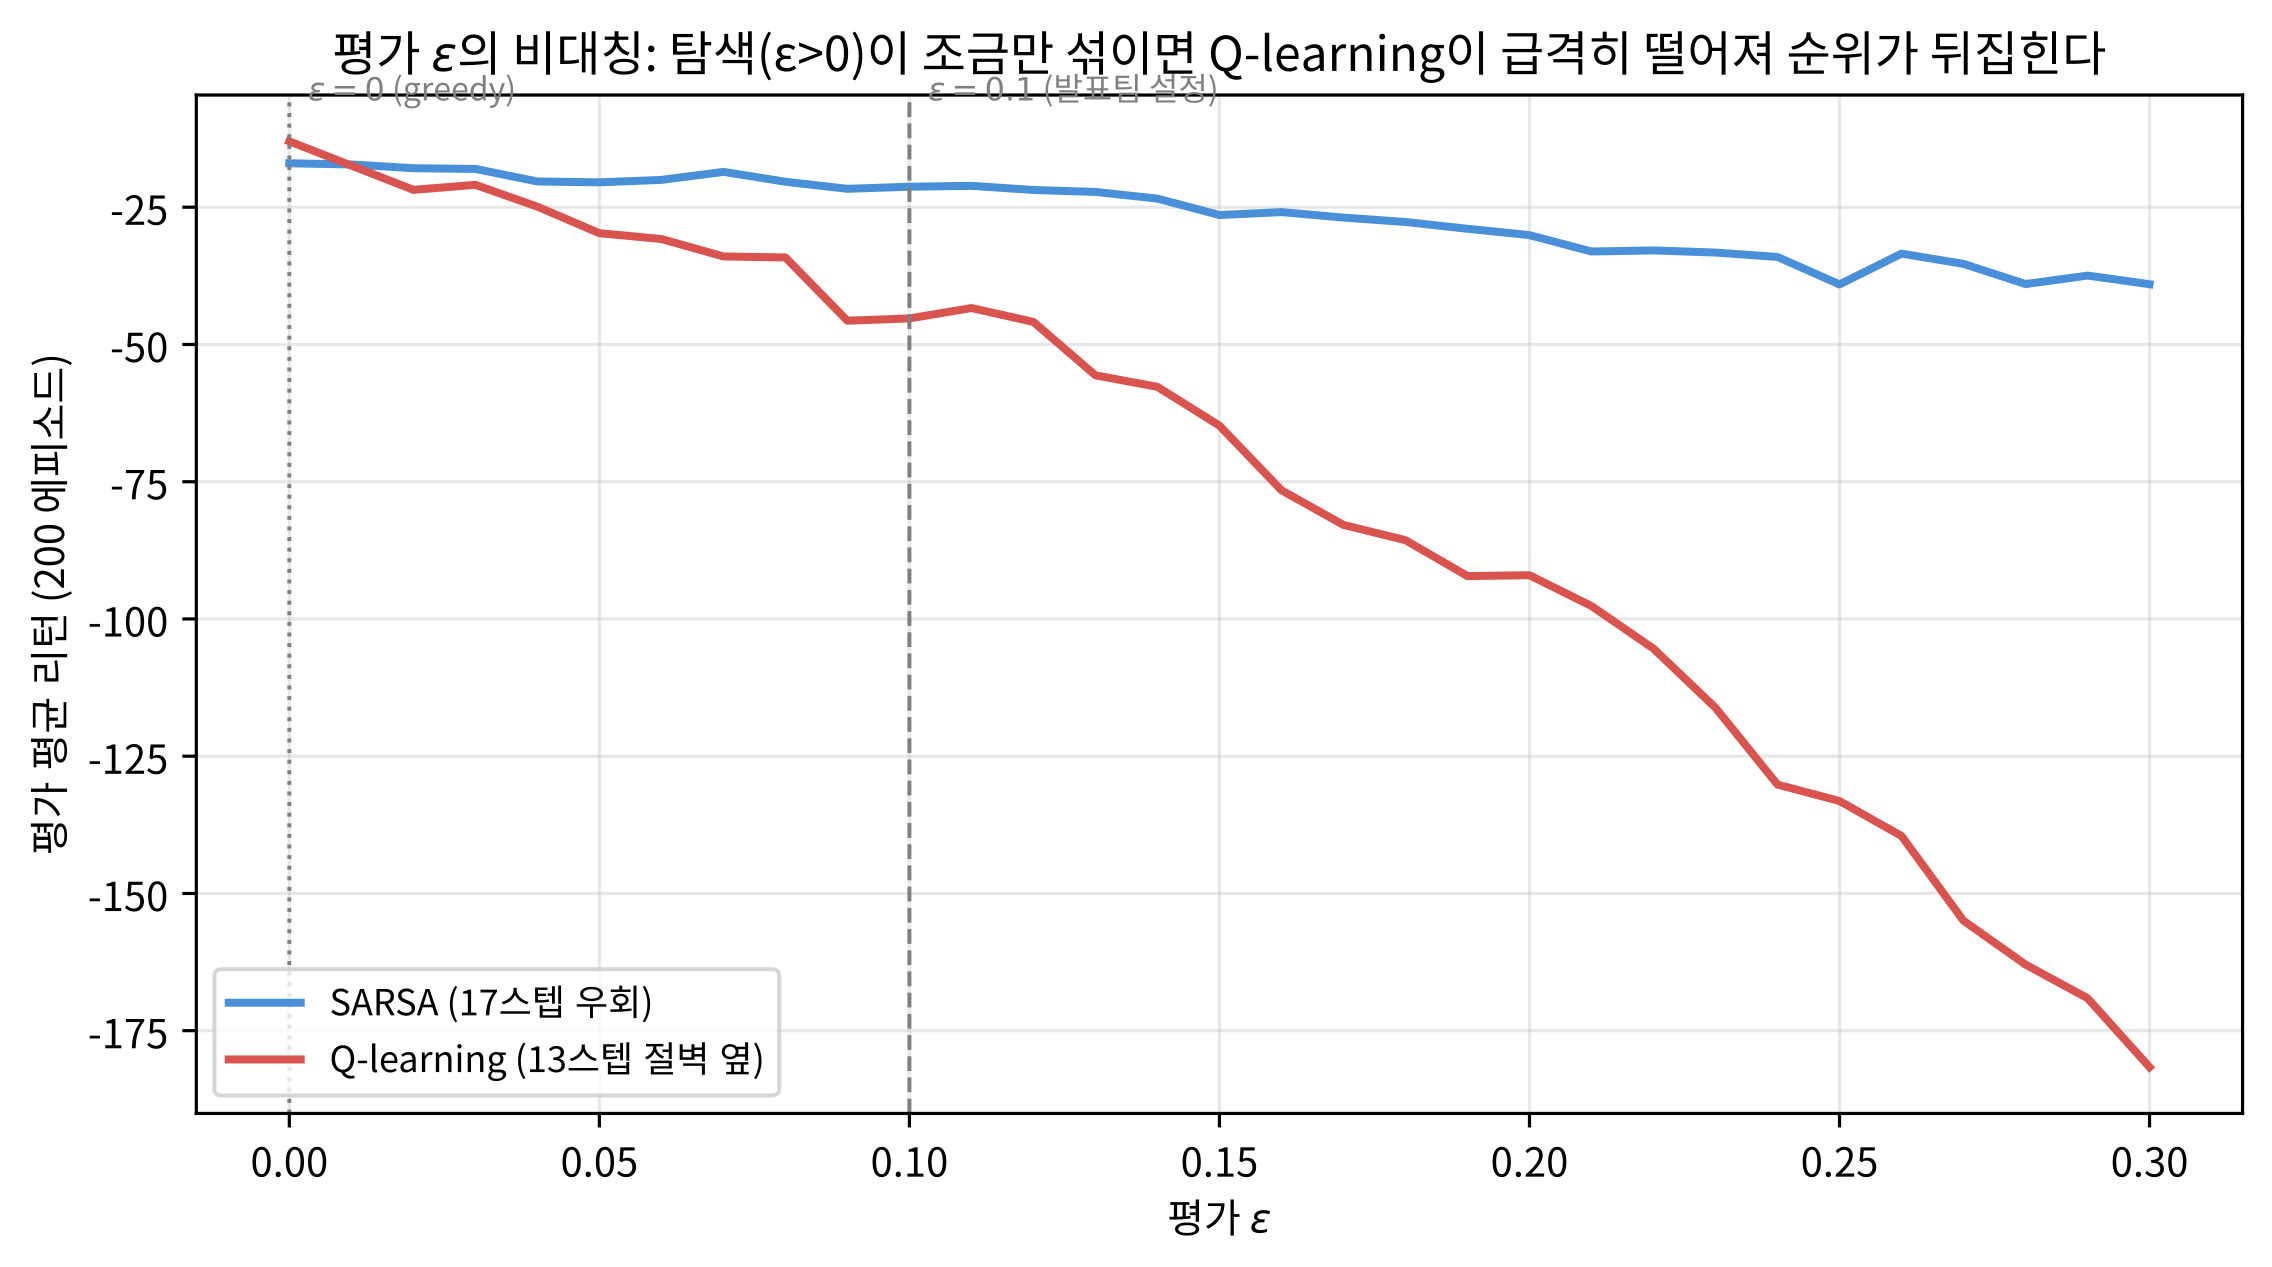
\includegraphics[width=\linewidth]{ch08_2_eval_epsilon_asymmetry.png}
      \vskip0.3em
      {\footnotesize $\varepsilon=0\sim0.3$으로 200 에피소드 평가.
      $\varepsilon=0$이면 Q 앞선다($-13$ vs $-17$)가, 탐색이 조금만
      섞이면 Q 급락($\varepsilon=0.1\to -45$, $0.3\to -182$)해 SARSA가
      뒤집어 앞선다. SARSA 우회 경로는 거의 안 흔들림($-17\to -39$).}
    \end{column}
    \begin{column}{0.4\textwidth}
      \begin{block}{핵심 태도}
        \textbf{리뷰어는 발표팀의 실험을 \emph{자기 손으로} 재실행할
        수 있는 사람.} ``이 학습 곡선, 시드를 바꿔서 다시 돌려도
        같은 모양이 나올까요?''라는 질문은 \textbf{리뷰어가 실제로
        다시 돌려본 적 있는} 질문일 때 가장 날카롭다.
      \end{block}
      \vskip0.4em
      {\footnotesize ``평가 때 $\varepsilon$을 켜둔 채'' 비교하면
      \textbf{결론의 방향이 뒤집히는} 구조.}
    \end{column}
  \end{columns}
\end{frame}

\begin{frame}{좋은 리뷰를 쓰는 과정: 체크리스트 $\to$ 반박 가능한 질문}
  \begin{columns}[T]
    \begin{column}{0.5\textwidth}
      \centering
      % [fig missing] \includegraphics[width=\linewidth]{ch08_2_rl_review_flow.png}
      \vskip0.3em
      {\footnotesize 발표+보고서로 주장 파악 $\to$ 4항목 적용 $\to$
      각 항목에 질문 초안(답이 \textbf{새로운 계산·실험}이어야 함)
      $\to$ ``개념(장·절)을 근거로 들고, 답이 새 실험인가?'' 분기: 예 $\to$
      \textbf{채택}, 아니오 $\to$ 감상평으로 떨어지고 다시 쓰기 $\to$
      3단계(1/2/3점)로 자기 채점.}
    \end{column}
    \begin{column}{0.48\textwidth}
      \begin{itemize}
        \item 흐름: 발표를 듣고 $\to$ 4항목에 적용 $\to$ 각 항목에서
          \textbf{구체적 관찰}을 적고 $\to$ 이 학기 개념(장·절)에
          뿌리를 박은 질문인지 검사 $\to$ 아니면 \textbf{다시 쓰기}.
        \item RL 버전의 특징: ML1 템플릿에서 \textbf{5번을 두 칸으로
          늘림} --- ``근거가 되는 \textbf{개념}'' + ``반박하려면 어떤
          \textbf{새 실험}이 필요한지''.
        \item 답이 \textbf{새 실험}이어야만 질문이 3점.
      \end{itemize}
    \end{column}
  \end{columns}
\end{frame}

\begin{frame}{리뷰 템플릿 (5번의 두 칸이 핵심)}
  \scriptsize
  \begin{tabular}{@{}p{0.16\textwidth}p{0.8\textwidth}@{}}
    \toprule
    칸 & 내용 \\
    \midrule
    1. 환경 설명 & 상태·행동·보상·주 지표(greedy 평가 리턴? 학습중 리턴?)가
      보고서에서 추적 가능한가? \textbf{베이스라인(무작위) 리턴}은
      명시됐는가? \\
    2. 알고리즘 선택 & 이 환경의 어떤 특성(상태 수, 보상 구조, 확률 전이)
      이 비교를 정당화하는가? 그 연결이 Ch\,4$\sim$7 개념으로
      설명되는가? \\
    3. 수식적 정당화 & ``$\geq 1$개''(8.1)를 채웠는가? 짚은 개념이
      \textbf{실제로 관측한 숫자}와 일치하는가(단순 인용이 아닌가)? \\
    4. 결과의 정직성 & 시드 $\geq 3$, 시드별 숫자 표, 평가 프로토콜
      ($\varepsilon=0$? 에피소드 수?) 명시. 불안정한 시드·구간이
      \textbf{정직하게} 보고됐는가? \\
    5. \textbf{반박 가능한 질문(필수, 1개 이상)} &
      \textbf{근거가 되는 개념}: Chapter \_\_ 절 \_\_ (개념: \_\_\_) \quad
      \textbf{발표팀이 답하려면 필요한 새 실험/계산}: \_\_\_ \quad
      \textbf{질문}: \_\_\_ (발표팀이 \emph{답이 나쁘면} 결과가
      흔들리는 것이어야) \\
    \bottomrule
  \end{tabular}
  \vskip0.6em
  \begin{block}{3점 도달 조건}
    5번의 ``개념''과 ``새 실험'' \textbf{두 칸이 모두} 채워져야 3점.
    둘 중 하나가 비어 있으면 \textbf{반박 불가능}한 리뷰.
  \end{block}
\end{frame}

\begin{frame}{자주 하는 실수: 학습 곡선 한 번만 보고 결론 내리기}
  \begin{itemize}
    \item RL에서 특히 부실한 리뷰: ``곡선이 잘 올라갔으니 성공''.
      먼저 물어야 할 것:
    \begin{itemize}
      \item 그 곡선이 \textbf{무작위 시드 하나}만 돌린 결과인가,
        여러 번 반복해 \textbf{일관된 경향}인가?
      \item $\varepsilon$이 충분히 감소했는가(또는 고정된 채 \textbf{최종
        정책 평가까지 탐험이 섞여} 있지는 않은가)?
    \end{itemize}
    \item 구조적으로 더 위험한 이유: 곡선의 ``오르다/안 오르다''가
      \textbf{학습의 진전과 분리될 수 있기 때문}.
  \end{itemize}
  \vskip0.5em
  \begin{block}{Montezuma's Revenge (DQN, 2015; R2D2, 2019)}
    DQN 에이전트는 수백만 스텝을 학습해도 \textbf{점수가 거의 0}에
    머물러 ``아무것도 배우지 못한다''고 판단됐고, 2019년 모델 기반
    R2D2가 처음 풀었을 때 ``점수 0''이 난이도/방법의 한계였음이
    확인됨. \kq{하나의 지표가 평탄했다만으로는 ``배우지 못했다''를
    결정할 수 없다.}
  \end{block}
\end{frame}

\begin{frame}{학습 곡선 3문: 리뷰어가 던지는 질문}
  \begin{center}
    \begin{block}{곡선을 보고 던져야 할 질문 3가지}
      \begin{enumerate}
        \item \textbf{시드} --- 이 곡선은 시드 \textbf{몇 개의 평균(또는
          시드별 범위)}인가요? 시드 1개라면 ``일관된 경향''을 말할
          수 없다.
        \item \textbf{$\varepsilon$ 스케줄} --- 학습 도중 $\varepsilon$이
          \textbf{어떻게 변했나요}? 평가 때 $\varepsilon=0$이었나요?
        \item \textbf{지표 분리} --- 곡선이 ``학습 \textbf{중} 리턴''인지
          ``학습 \textbf{후} 평가 리턴''인지? 둘은 \textbf{다른 대상}의
          측정값이다(8.1 §비교 프로토콜).
      \end{enumerate}
    \end{block}
  \end{center}
  \vskip0.5em
  {\footnotesize ``곡선이 평탄해서 못 배운 것 같다''(1점 인상평) 대신,
  ``그 평탄한 구간에서 \textbf{에피소드 길이}나 \textbf{보이지 않는
  중간 지표}(특정 구역 도달 여부, Q값의 변화)는 개선됐나요? 평탄한 것이
  \textbf{측정하지 않은 지표} 때문은 아닌가요?''(3점)로 번역하는 것.
  3문 = §5가지 패턴 1·2번 + 8.1 §비교 프로토콜의 리뷰어 언어 압축.}
\end{frame}

\begin{frame}{우리 팀 발표를 리뷰하기: 발표 전 셀프-리뷰}
  \begin{itemize}
    \item 최선의 전략: \textbf{네가 심사할 때 던질 수 있는 가장
      날카로운 질문을, 네 발표 \emph{전에} 스스로 던져보고 답을
      준비해두는 것}.
    \item §5가지 패턴의 5개 질문을 자기 팀 보고서에 적용:
    \begin{itemize}
      \item (1) 시드 3개 greedy 평가 \textbf{표}가 보고서에 있는가?
      \item (2) \textbf{평가 프로토콜 문장}($\varepsilon=0$, 200
        에피소드, 모든 알고리즘·시드에 동일)이 있는가?
      \item (3) 무작위 정책 리턴이 \textbf{실측 숫자}로 적혀 있는가?
      \item (4) $\alpha$·$\varepsilon$ 민감성을 \textbf{한 줄이라도}
        검토했는가?
      \item (5) 불안정한 시드·구간이 ``잘 안 된 부분'' 절에
        \textbf{사라지지 않고} 있는가?
    \end{itemize}
  \end{itemize}
  \vskip0.5em
  \begin{block}{왜 발표 \emph{전}인가}
    이 5가지에 답이 없다면, 발표 전에 해결해두는 것이 발표 중에
    3점 리뷰를 받는 것보다 \textbf{항상 낫다}. Block B Ch\,16.1도
    동일한 구조(발표 $\to$ peer-review) --- 이 셀프-리뷰 습관이
    학기 말까지 이어진다.
  \end{block}
\end{frame}

\begin{frame}{확인 문제 (1/2): 리뷰어가 될 때의 판단력}
  \small
  \begin{block}{Q1. ``시드 3개를 돌려 greedy가 $-13/-14/-12$로 Q-learning이
  안정적이다'' --- 이 편차는 \emph{무엇의} 편차이고, \emph{무엇의}
  편차가 \emph{아니}인가}
  \begin{itemize}
    \item 세 숫자 = \textbf{세 개의 서로 다른 정책}의 greedy 평가
      (학습 과정의 무작위성/시드가 만든) --- ``어떤 정책이 학습됐는가''
      의 편차이지, ``그 정책을 재는 \textbf{측정 오차}''가 아님.
    \item 평가 에피소드를 늘려도 \textbf{사라지지 않음}. 각 시드
      자체($-13$ 등)는 200 에피소드 측정의 평균이라 \textbf{그 시드의}
      측정 오차만 줄어듦.
    \item ``안정적이다''라 말하려면 \textbf{두 층을 구분}: ``시드 간
      편차 $\pm 1$, 각 시드 측정 오차 $\pm 0.x$''.
  \end{itemize}
  \end{block}
  \vskip0.4em
  \begin{block}{Q2. ``학습에 $\varepsilon=0.1$ 쓰고, 최종 평가는 \emph{학습된
  정책으로} 200 에피소드''의 모순}
  \begin{itemize}
    \item $\varepsilon=0.1$이면 매 스텝 10\% 확률로 무작위 $\to$
      ``학습된 정책으로''도 \textbf{탐험이 섞인} 측정.
    \item CliffWalking에서 이는 \textbf{결론의 방향을 가름}:
      $\varepsilon=0.1$ 평가 $\to$ SARSA $-21.3$ vs Q $-45.3$(SARSA
      우위); $\varepsilon=0$ $\to$ Q $-13$ vs SARSA $-17$(\textbf{순수
      역전}). 질문: ``최종 평가가 $\varepsilon=0$(greedy)였나요?
      $\varepsilon=0.1$으로 재평가하면 순위가 뒤집힙니다(Ch\,6.3) ---
      두 프로토콜 모두로 시드 3개를 재실행해주세요.''
  \end{itemize}
  \end{block}
\end{frame}

\begin{frame}{확인 문제 (2/2): 2점 $\to$ 3점으로 바꾸기}
  \small
  \begin{block}{Q3. ``Q-learning이 off-policy라 SARSA보다 높았다.
  이는 Ch\,6.3 이론과 일치한다''로 끝난 정당화}
  \begin{itemize}
    \item \textbf{2점} --- 개념(Ch\,6.3)은 인용했지만 \textbf{관측
      숫자가 없고} 발표팀이 ``네, 이론이 맞습니다''로 넘길 수 있음.
    \item 3점 변환(\textbf{관찰 + 개념 + 왜 문제인지}): ``off-policy
      라는 설명은 \emph{학습 도중} 리턴(SARSA $-24$ vs Q $-49$)에는
      \textbf{반대 방향}을 예측 --- 절벽 옆 경로는 탐험 한 번이 $-100$이라
      학습중에는 \emph{더 낮게} 나와야. greedy($-13$ vs $-17$)가 높다는
      것만으론 \emph{경로 길이} 차이일 수 --- 13스텝 vs 17스텝으로
      연결한 설명이 있습니까?''
  \end{itemize}
  \end{block}
  \vskip0.4em
  \begin{block}{Q4. ``왜 $\gamma=1.0$인가요? 0.95로 하면?''이 3점인가}
  \begin{itemize}
    \item 이대로는 \textbf{2점} --- $\gamma$는 하이퍼파라미터가 아니라
      \textbf{MDP의 정의}(Ch\,3.1 5요소)에 속함. ``왜 $\gamma=1.0$?''은
      ``왜 이 문제를 풀어요?''에 가까워 \textbf{문제 정의}의 문제.
    \item 같은 의도의 3점: ``여러분이 \textbf{해결하려는 문제}가 할인율에
      민감한가요? $\gamma=0.95$로 바꾸면 greedy 정책의 경로가 달라지는데,
      이 환경에서 $\gamma=1.0$이 자연스러운가 --- 그 선택이 8.1
      ``문제 정의'' 절에 근거와 함께 명시됐나요?'' $\to$ 체크리스트
      \textbf{1번(문제 정의)}으로 연결되는 개념 있는 질문.
  \end{itemize}
  \end{block}
\end{frame}

\begin{frame}{확인 문제 Q5 + 자주 묻는 질문}
  \small
  \begin{block}{Q5. ``시드 3개: SARSA $-17/-17/-17$, Q $-13/-13/-13$.
  Q-learning이 더 좋다'' $\to$ 리뷰어 ``Q-learning이 \emph{항상} 더
  좋은가요?''}
  \begin{itemize}
    \item \textbf{정직한 범위}: ``이 환경·이 설정($\alpha$, $\varepsilon$
      스케줄, 500 에피소드)에서 시드 3개로 확인한 한도에서 Q의 greedy
      평가가 앞선다''. 이 실험 \textbf{외부}로(다른 환경·$\alpha$$\cdot$
      스케줄)의 일반화는 지지되지 않음.
    \item \textbf{말하지 말아야 할} 추론: ``Q-learning이 \emph{더 좋은
      알고리즘}이다'' --- 이 비교는 \emph{탐욕적 실행 시} 어느 정책이
      나은가의 답이지 알고리즘 우열의 답이 아님(학습중에는 SARSA가
      앞서며, 6.3절 on/off-policy 차이로 설명).
  \end{itemize}
  \end{block}
  \vskip0.3em
  {\footnotesize
  \textbf{FAQ} --- (a) 하이퍼파라미터 선택 근거까지 물어보는가? \textbf{그렇다},
  ``적당히'' 고른 값이 결과에 얼마나 큰 영향(Ch\,7.2 n 튜닝)을 주는지
  = 방법론 적절성의 핵심. (b) ``문제 없이 잘한 팀''에서 3점 질문?
  ``\emph{보이지 않는} 것 $\neq$ \emph{확인되지 않은} 것 --- 3점은 항상
  \textbf{확인되지 않은 영역}(시드 5개, $\alpha$ 민감성, 다른 평가
  프로토콜)에서. (c) 발표팀이 그 자리에서 답 못 하면 점수? \textbf{리뷰어
  점수(질문 품질)와 발표팀 점수는 따로} --- 리뷰어는 질문을, 발표팀은
  답을. (d) 결과가 정말 나빴던 팀? \textbf{``나쁜 결과''는 좋은 리뷰의
  대상} --- ``그 \emph{진단}이 Ch\,4$\sim$7 개념으로 타당하나요?''
  방법론만 보고, 사람은 보지 않는 것. (e) 10분뿐인데? 4항목 \emph{모두}에
  3점 질문이 \textbf{아님} --- 4항목 다 확인 후 \textbf{가장 날카로운
  질문 1개}를 5번 칸에. 시간이 부족하면 ``실험 프로토콜의 정직성''(시드,
  평가 $\varepsilon$, 베이스라인)을 \textbf{먼저} --- 이 결함은 뒤의
  결과 해석 전체를 흔듦.}
\end{frame}

\section{8.3 중간고사 대비 총정리}

\begin{frame}{이 절: 새 개념 0개, 하는 일 세 가지}
  \begin{itemize}
    \item (1) Ch\,2$\sim$7 이론을 \textbf{``손으로 재현할 수 있는
      형태''}로 압축.
    \item (2) 준비도를 스스로 재는 \textbf{자가진단} 제시.
    \item (3) 8.1에서 4주간 쌓아온 프로젝트 절차를 복습 자료로 재작성.
  \end{itemize}
  \vskip0.6em
  \begin{block}{시험의 성격}
    시험은 \textbf{``Block A의 개념을 \emph{새로운 MDP}에 적용하는
    것''}이므로, \textbf{암기는 쓸모가 없고} 이 절은
    \textbf{``스스로 유도하는 습관''} 하나에 맞추어져 있다.
  \end{block}
  \vskip0.6em
  {\footnotesize 특히 ``벨만방정식을 터미널부터 거꾸로 대입해 직접
  풀기''(Ch\,4)와 ``TD 오차의 수렴 조건 논증''(Ch\,6)이 다른 MDP에도
  그대로 적용되는지가 좋은 복습.}
\end{frame}

\begin{frame}{장별 핵심 질문 (Ch\,2$\sim$7)}
  \scriptsize
  \begin{tabular}{@{}clp{0.6\textwidth}@{}}
    \toprule
    장 & 핵심 질문 & 다시 볼 개념 \\
    \midrule
    Ch\,02 & 상태 없이도 탐험-활용 딜레마가 있는가 & $\varepsilon$-greedy,
      낙관적 초기화, UCB \\
    Ch\,03 & RL 문제를 어떻게 수학적으로 정식화하는가 & MDP 5요소,
      마르코프 성질, 할인율 \\
    Ch\,04 & 모델을 알 때 최적 정책을 어떻게 계산하는가 & 벨만방정식,
      정책반복/가치반복, 축소 사상 \\
    Ch\,05 & 모델 없이 에피소드 결과만으로 배울 수 있는가 & 첫방문 MC,
      MC 제어, 중요도 샘플링 \\
    Ch\,06 & 에피소드가 끝나길 기다리지 않고 배울 수 있는가 & TD 오차,
      Q-learning vs SARSA \\
    Ch\,07 & MC와 TD 사이, 경험 재사용은 어떻게 하는가 & n-step TD,
      적격흔적, Dyna-Q \\
    \bottomrule
  \end{tabular}
  \vskip0.8em
  \begin{block}{시험 형식 (참고)}
    100분, 4문항 --- ① 템플릿 ①(거꾸로 대입)을 새 MDP에 적용, ②
    벨만방정식·정책반복 유도/수렴 논증, ③ MC/TD 갱신 규칙의 수치
    계산(경로 따르기), ④ 개념 비교 단답(SARSA vs Q, 편향-분산,
    on/off-policy). \kq{모든 문항은 계산 과정을 보여야 한다} ---
    최종 답만 맞고 과정 없으면 과정이 맞던 지점까지만 부분점.
  \end{block}
\end{frame}

\begin{frame}{유도 템플릿 ①: 거꾸로 대입 (backward induction)}
  \begin{itemize}
    \item \kb{뼈대}: 전이가 ``앞으로만'' 흐르는 MDP에서 벨만방정식
      $V^\pi(s)=R(s,\pi(s))+\gamma V^\pi(s')$를 \textbf{터미널에서
      출발해 거꾸로 한 칸씩 대입}하면 \textbf{연립방정식을 풀지 않아도}
      풀린다.
    \item \kb{왜 동작하나}: 전이 그래프가 \textbf{사이클 없이 한 방향}
      (0$\to$1$\to$2 사슬, 유한 스텝 후 ``끝'' 보장)이면 연립방정식의
      마지막 줄이 더 이상 다른 상태를 참조하지 않음 $\to$ 해가 터미널
      에서 ``퍼져 나간다''. (Ch\,3 3칸 보드게임, Ch\,5 블랙잭, 7.3의
      5$\times$5 격자)
  \end{itemize}
  \vskip0.5em
  \begin{block}{작은 예제: 3-state 사슬, $\gamma=0.9$ (0$\to$1: $-1$,
  1$\to$2: $-1$, 2=터미널)}
    \[
      V(2)=0 \ \text{(터미널)} \qquad
      V(1)=-1+0.9\,V(2)=-1 \qquad
      V(0)=-1+0.9\,V(1)=-1.9
    \]
    \textbf{정확성 확인}(답안에 한 줄): $V=(-1.9,-1,0)$를 벨만방정식
    \textbf{양변에 다시 대입}해 좌우가 일치하는가?
  \end{block}
  \vskip0.4em
  {\footnotesize \textbf{자주 하는 실수} --- (1) 터미널 진입 보상 자체를
  빼먹기, (2) \textbf{대입 방향을 거꾸로} 쓰기($V(1)=-1+0.9V(0)$로).
  대입 방향은 ``다음 상태의 값이 \emph{이미 알려진} 쪽'' = 전이 화살표와
  \textbf{반대}.}
\end{frame}

\begin{frame}{유도 템플릿 ②: 후보+검증 (candidate \& verify) — 뼈대·해}
  \begin{itemize}
    \item \kb{뼈대}: (1) 최적값의 \textbf{후보} 추측, (2) 그 후보가
      성립한다고 \emph{가정하고} 방정식 풀기, (3) 각 상태에서 후보
      행동이 \emph{정말로} 다른 행동보다 나은지 \textbf{검증}.
    \item 벨만 \textbf{최적}방정식 $Q^*(s,a)=R+\gamma \max_{a'}Q^*(s',a')$
      의 $\max$는 ``argmax인 행동을 모르면 펼칠 수 없는'' 함수
      $\to$ \textbf{검증이 선택이 아니라 필수}.
  \end{itemize}
  \vskip0.4em
  \begin{block}{작은 예제 (강의에서 안 써본 \emph{새} MDP, $\gamma=0.9$)}
    상태 S, G, T. S: ``run''은 0.7 확률로 G, 0.3 확률로 S로 미끄러짐
    (보상 0); ``rest''는 S에 남음(보상 $-1$). G: ``collect''로 T(보상
    $+3$). T=터미널.
    \begin{itemize}
      \item \textbf{Step 1 (후보)}: $+3$의 유일한 길 = G에서 collect
        $\to$ $Q^*(G,\text{collect})=3$. S에서 rest는 매 스텝 $-1$
        $\to$ 후보: \textbf{run@S, collect@G}.
      \item \textbf{Step 2 (해)}: run@S 가정 하에
        $V^*(S)=0.9\big(0.7\,V^*(G)+0.3\,V^*(S)\big)=1.89+0.27\,V^*(S)$
        --- 자기 자신으로 돌아오는 확률 $0.9\times 0.3=0.27$ 때문에
        \[
          V^*(S)=\frac{1.89}{1-0.27}=\frac{189}{73}\approx 2.589
        \]
    \end{itemize}
  \end{block}
\end{frame}

\begin{frame}{유도 템플릿 ②: 검증이 안전장치인 이유}
  \begin{block}{Step 3 (검증): run이 정말 rest보다 나은가}
    \[
      Q^*(S,\text{run})=2.589 \;>\;
      Q^*(S,\text{rest})=-1+0.9\times 2.589=1.330 \;\;\checkmark
    \]
    일치 $\to$ 후보 성립, 답: $V^*(S)=2.589$, $V^*(G)=3$.
  \end{block}
  \vskip0.4em
  \begin{itemize}
    \item \textbf{Step 3은 형식이 아니라 안전장치} --- Step 1의 추측이
      틀렸다면 Step 2의 값은 ``틀린 정책을 최적인 것처럼 놓고 푼 값'',
      Step 3의 부등호가 뒤집힘. (계산이 $Q(\text{rest})=3.5>Q(\text{run})$
      이었다면 = ``\textbf{후보가 틀렸으니 다시 추측하라}''는 신호.)
  \end{itemize}
  \vskip0.5em
  \begin{block}{정책반복(Ch\,4.2)과의 연결}
    이 템플릿은 ``improve + evaluate'' 루프를 \textbf{손으로 단축}한 것.
    $\pi_0=\text{rest@S}$로 시작했다면 정책평가 $V^\pi(S)=\frac{-1}{1-0.9}=-10$,
    improve에서 $Q^\pi(S,\text{run})=0.9(2.1+0.3\times(-10))=-0.81>-10$
    으로 run 교체, 재평가에서 다시 2.589 --- \textbf{1회 반복에 같은
    답}. ``후보 추측은 정책반복을 손으로 건너뛰는 단축키''를 시험에서
    말하면 이 템플릿은 끝.
  \end{block}
\end{frame}

\begin{frame}{유도 템플릿 ③: 축소 사상 $\to$ 기하급수 감소}
  \small
  \begin{block}{뼈대 (``T는 $\gamma$-축소 사상''이 주어졌을 때)}
    \begin{enumerate}
      \item 오차를 $\|V_n-V^*\|$ 로 표기.
      \item $V^*$가 고정점 $\to$
        $\|V_n-V^*\|=\|TV_{n-1}-TV^*\|\le \gamma\,\|V_{n-1}-V^*\|$.
      \item $n$번 반복: $\|V_n-V^*\|\le \gamma^n\|V_0-V^*\|$.
      \item $\gamma<1 \Rightarrow \gamma^n\to 0$ $\to$ \textbf{수렴}.
    \end{enumerate}
  \end{block}
  \vskip0.4em
  \begin{itemize}
    \item \kb{왜 표준인가}: 4.3절 빈칸채움 폴백이 정확히 이 4줄. Ch\,6
      TD(0)/Q-learning 수렴 논증도 \textbf{같은 뼈대}에 조건 교체 ---
      ``TD 오차 0인 Q'' $\leftrightarrow$ ``고정점'', ``$\alpha$
      충분히 작고 모든 (s,a) 무한 방문''이 축소 조건 역할(확률적
      설정은 \textbf{기댓값에서만} 축소 성립 --- Ch\,06 FAQ 복습).
    \item \textbf{자주 하는 실수}: Step 2에 쓸 ``$V^*$는 고정점''
      \textbf{전제를 잊음} --- 없으면 $TV_{n-1}-TV^*$를 처리할 근거
      없음. Q-learning 버전은 6.3절 연습문제 3의 \textbf{세 조건}
      ($\alpha$ 충분히 작음, 모든 (s,a) 무한 방문, TD 오차 0 $\Leftrightarrow$
      벨만 최적방정식의 해)을 빠뜨리지 않는 것이 채점 기준.
  \end{itemize}
\end{frame}

\begin{frame}{숫자 감각: $\gamma=0.9$인 기하급수 감소}
  \begin{columns}[T]
    \begin{column}{0.5\textwidth}
      \small
      \begin{tabular}{@{}clp{0.4\textwidth}@{}}
        \toprule
        반복 수 $n$ & $\gamma^n$ & 뜻 \\
        \midrule
        5 & 0.590 & 초기 오차의 59\% 이하로 \\
        10 & 0.349 & \\
        20 & 0.122 & 약 1/8 \\
        50 & 0.0052 & 초기 오차의 99.5\%가 사라짐 \\
        \bottomrule
      \end{tabular}
      \vskip0.6em
      {\footnotesize ``오차가 1\% 이하가 되기까지 몇 번?'' =
      $\gamma^n<0.01$ 을 $n$에 대해 풀기:
      $n>\ln 0.01/\ln 0.9\approx 44$ 번.}
    \end{column}
    \begin{column}{0.46\textwidth}
      \begin{block}{시험에서 쓰는 한 줄}
        ``$\gamma$-축소 사상 + 고정점 + $\gamma<1$ 이 주어지면,
        오차는 $\gamma^n$ 배로 기하급수 감소해 \textbf{임의 초기값에서
        수렴}한다.''
        --- 이 3개 전제(축소, 고정점, $\gamma<1$)를 \textbf{모두}
        명시해야 논증 완성.
      \end{block}
    \end{column}
  \end{columns}
  \vskip0.5em
  {\footnotesize 3가지 템플릿(거꾸로 대입 / 후보+검증 / 축소 사상 수렴)이
  시험 손유도 문항의 \textbf{전부}를 덮는다 --- 뼈대를 외우는 것이
  아니라 \textbf{각 뼈대의 빈칸을 스스로 채우는 것}이 목표.}
\end{frame}

\begin{frame}{Block A 개념 지도: 한 질문에 여섯 각도}
  \begin{itemize}
    \item 여섯 장 = \textbf{``미래의 불확실한 보상을 지금 어떻게
      수치화할 것인가''라는 한 질문에 여섯 가지 각도}에서 답한 것.
      복습 = 주제 6개 훑기가 아니라 \textbf{답들 사이의 관계}를 다시
      그리는 일.
    \item 구조: 위 = 문제 정식화(Ch\,2$\sim$3: 밴딧 $\to$ MDP 5요소
      $\to$ 리턴/할인율). 가운데 = 4가지 경로 --- 모델 기반
      (벨만 $\to$ 정책반복/가치반복, Ch\,4) vs 모델 프리
      (MC Ch\,5 $\to$ TD Ch\,6 $\to$ n-step·적격흔적·Dyna-Q Ch\,7).
      아래 = 모든 경관을 가로지르는 \textbf{공통 축}: 편향-분산,
      탐험($\varepsilon$-greedy·낙관적 초기화·UCB), 수렴(목표값
      오차$\to$0, $\alpha$ 작게, 무한 방문), on/off-policy.
      오른쪽 = Block B(Ch\,9$\sim$16) 화살표: Q 표를 \textbf{신경망}
      으로(DQN), 로봇 시뮬레이션.
  \end{itemize}
  \vskip0.5em
  \begin{center}
    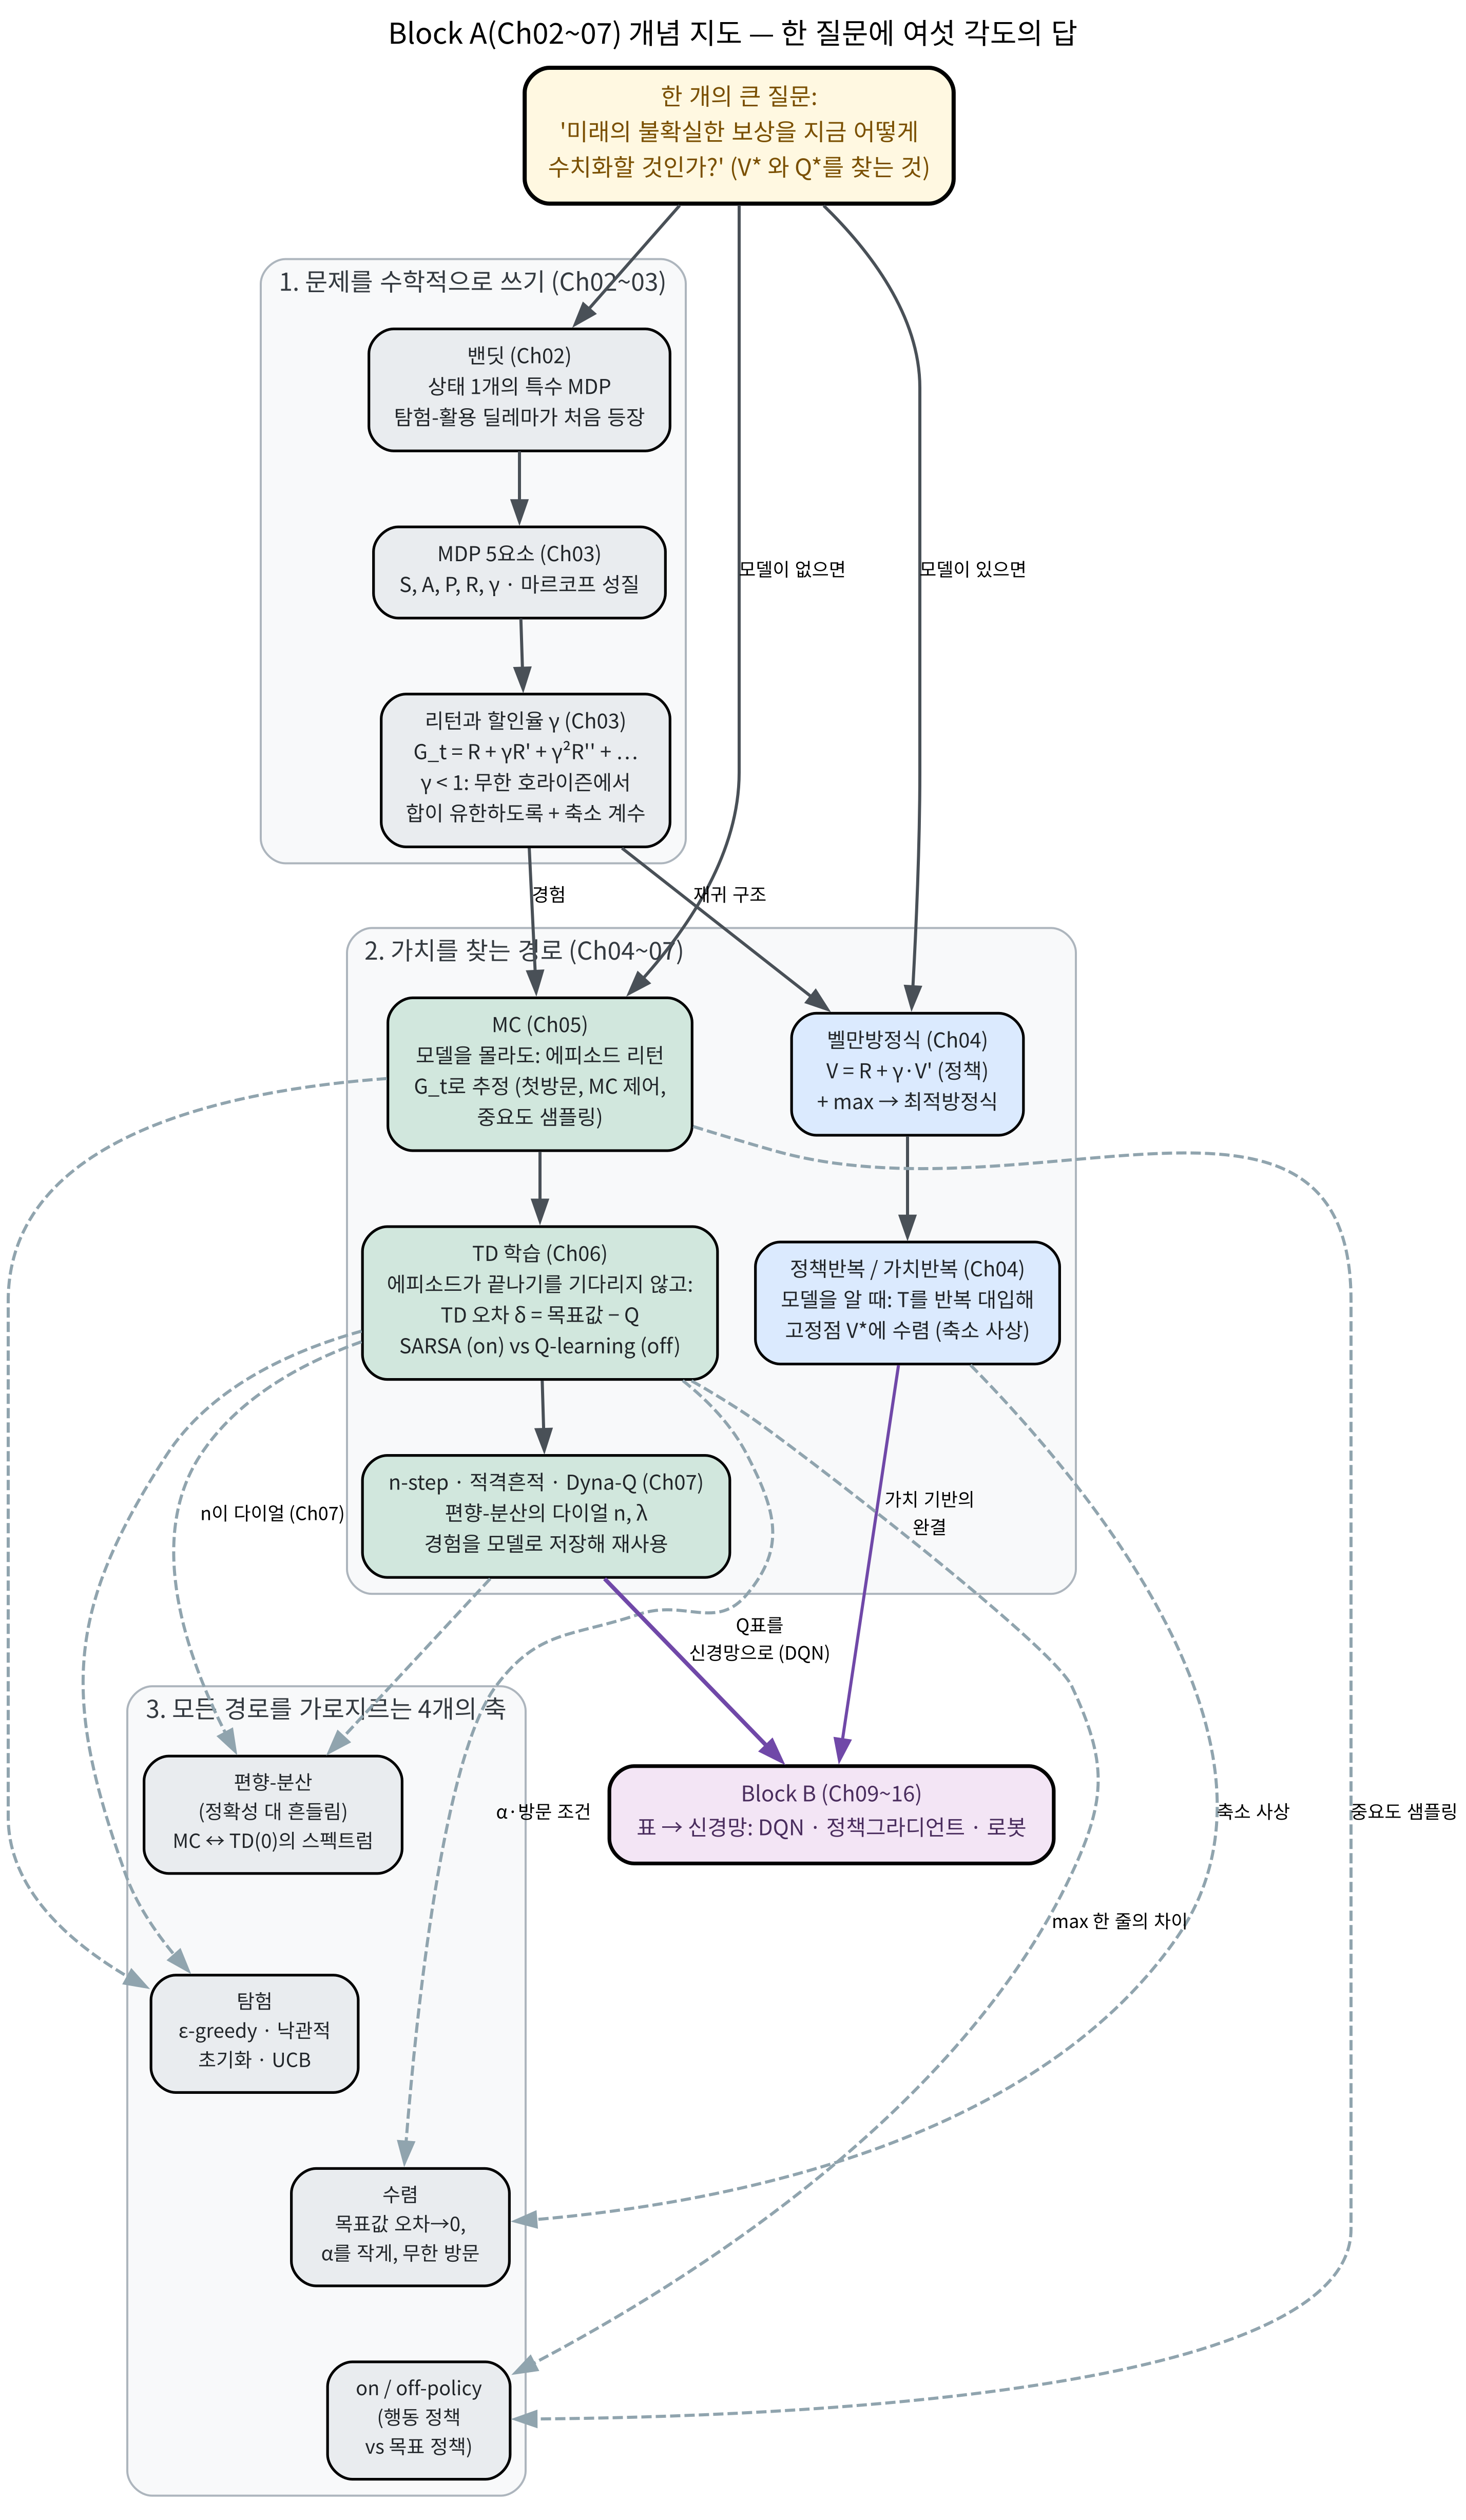
\includegraphics[width=0.72\linewidth]{ch08_3_rl_concept_map.png}
  \end{center}
\end{frame}

\begin{frame}{개념 지도를 읽는 법: 시험 기법 두 가지}
  \begin{columns}[T]
    \begin{column}{0.5\textwidth}
      \kb{(1) ``질문이 지도의 어디를 가리키는지''}
      \begin{itemize}
        \item ``SARSA는 on-policy인가'' = 가운데 행(TD 박스)과 아래
          행(on/off-policy 축)이 만나는 \textbf{엣지}.
        \item ``왜 $n=5$가 $n=1$보다 좋은가'' = n-step 박스와
          \textbf{편향-분산 축}의 엣지.
        \item ``어떤 박스와 어떤 축의 교차점인가''를 5초 안에 짚으면
          \textbf{답을 그 축의 용어로} 말할 수 있다.
      \end{itemize}
    \end{column}
    \begin{column}{0.5\textwidth}
      \kb{(2) ``엣지가 곧 '왜'다''}
      \begin{itemize}
        \item 박스(개념 \textbf{정의}) 자체를 묻는 문항은 드묾.
        \item 빈출 문항은 거의 전부 \textbf{엣지}: 왜 MC$\to$TD인가,
          왜 $\varepsilon$-greedy가 모든 박스에 붙는가, 왜 $\gamma$는
          1보다 작은가.
        \item \kq{박스는 외우기 쉬운데, \textbf{엣지가 시험}이다.}
      \end{itemize}
    \end{column}
  \end{columns}
  \vskip0.5em
  {\footnotesize 복습 우선순서는 시험 빈출 순서와 거의 같음: (1) MC$\to$TD,
  (2) TD $\leftrightarrow$ 편향-분산($n$의 다이얼), (3) TD
  $\leftrightarrow$ on/off-policy(SARSA vs Q), (4) MDP $\to$ 모든
  박스. 네 개를 한 문장씩 말할 수 있으면 지도는 끝.}
\end{frame}

\begin{frame}{확인 문제: 장을 넘나드는 복습 4개 (답)}
  \scriptsize
  \begin{tabular}{@{}p{0.34\textwidth}p{0.62\textwidth}@{}}
    \toprule
    질문 & 답 (핵심) \\
    \midrule
    1. Ch\,2 밴딧과 Ch\,3 MDP의 관계 & 밴딧 = \textbf{상태가 하나뿐}이고
      어떤 행동을 해도 같은 상태로 전이하는 \textbf{특수한 MDP}.
      탐험-활용 딜레마는 이 특수 경우에도 그대로, Ch\,5$\sim$6의
      $\varepsilon$-greedy = 그 전략의 MDP 전체 확장 \\
    2. 정책반복/가치반복(Ch\,4) vs MC/TD(Ch\,5$\sim$6)의 근본 차이 &
      Ch\,4는 전이확률 $P(s'|s,a)$를 \textbf{정확히 안다고 가정}하고
      벨만방정식을 반복 대입(모델 기반). Ch\,5$\sim$6은 $P$를 몰라도
      \textbf{실제 경험}으로부터 추정(모델 프리) --- 단, 둘 다
      ``벨만방정식이라는 \textbf{같은 재귀 구조}''에 기대 \\
    3. MC / TD(0) / n-step의 목표값을 편향-분산으로 한 줄 &
      MC: 실제 리턴 $G_t$를 그대로 $\to$ \textbf{편향 없으나 분산
      큰} / TD(0): 한 스텝 실제 + 추정치 $\to$ \textbf{분산 작으나
      편향 있는} / n-step: 그 사이($n$이 다이얼, U자 트레이드오프) \\
    4. SARSA vs Q-learning의 on/off-policy 구분이 실전에서 중요한 이유 &
      \textbf{학습이 실제 위험한 환경}에서 일어나면 학습 도중의 안전까지
      고려하는 \textbf{SARSA(on-policy)} 계열이 유리. \textbf{시뮬레이터}
      에서 충분히 학습하고 최종 배포만 중요하다면 목표 정책의 최적성을
      직접 배우는 \textbf{Q-learning(off-policy)}이 유리(Ch\,6.3) \\
    \bottomrule
  \end{tabular}
  \vskip0.5em
  \begin{block}{한 줄 요약}
    Ch\,2$\sim$7의 모든 알고리즘은 \textbf{``미래의 불확실한 보상을 지금
    어떻게 수치화할 것인가''}에 대한 답 --- 이제 이 질문에
    \textbf{신경망}을 결합해 표에 담을 수 없을 만큼 큰 문제로 나아갈
    차례.
  \end{block}
\end{frame}

\begin{frame}{복습 자가진단: 20문항 (10초에 한 문장) 1$\sim$10}
  \scriptsize
  \begin{tabular}{@{}clp{0.72\textwidth}@{}}
    \toprule
    \# & 장 & 한 문장 질문 \\
    \midrule
    1 & Ch\,02 & 밴딧에서 ``지금까지 몇 번 당겼는가''가 상태에 들어가야
      하는 이유는? \\
    2 & Ch\,02 & $\varepsilon$-greedy, 낙관적 초기화, UCB --- 각각 탐험을
      유도하는 방식 한 단어로 \\
    3 & Ch\,03 & MDP 5요소 중 보상함수를 제외한 네 가지를 쓰시오 \\
    4 & Ch\,03 & $\gamma<1$이 단순 편의가 아니라 \emph{필수}인 경우는? \\
    5 & Ch\,02$\to$03 & 밴딧과 MDP의 관계를 한 문장으로 \\
    6 & Ch\,04 & 벨만 \emph{방정식}과 벨만 \emph{최적}방정식의 차이를
      한 문장으로 \\
    7 & Ch\,04 & ``T는 $\gamma$-축소 사상이다''를 수식 없이 한 문장으로 \\
    8 & Ch\,04 & 모든 상태가 전이 한 번 만에 터미널에 닿는 MDP에서
      정책평가는 몇 번의 반복이면 끝나고 왜? \\
    9 & Ch\,05 & 첫방문 MC가 왜 편향 없는가? \\
    10 & Ch\,05$\to$06 & MC 제어와 SARSA는 갱신하는 ``목표값''이 어떻게
      다른가? \\
    \bottomrule
  \end{tabular}
  \vskip0.5em
  {\footnotesize 기준: \textbf{10초 안에 한 문장}으로 답할 수 있으면 O,
  막히면 ✗. 18개 이상 = 준비 완료, 15$\sim$17 = ✗가 모인 장 위주로
  ``자주 하는 실수''+확인 문제 재독, 12$\sim$14 = §유도 템플릿 3가지
  손으로 재풀기, 12 미만 = §복습 주간 일정을 \textbf{건너뛰지 않기}.}
\end{frame}

\begin{frame}{복습 자가진단: 11$\sim$20 + 답 (한 줄)}
  \scriptsize
  \begin{tabular}{@{}clp{0.72\textwidth}@{}}
    \toprule
    \# & 장 & 한 문장 질문 \\
    \midrule
    11 & Ch\,05/06 & MC와 TD(0)의 목표값을 각각 \textbf{수식}으로 \\
    12 & Ch\,06 & ``TD 오차가 0''이 ``벨만방정식을 만족한다''와 같은
      말인 이유는? \\
    13 & Ch\,06 & SARSA와 Q-learning의 차이를 한 문장으로 \\
    14 & Ch\,06 & CliffWalking에서 ``더 짧은 경로''를 배운 알고리즘은?
      학습중 리턴이 오히려 더 나쁜 이유는? \\
    15 & Ch\,07 & n-step 리턴 $G_t^{(n)}$을 수식으로, $n=1$과
      $n=\infty$(유한)는 무엇으로 퇴화하는가? \\
    16 & Ch\,07 & 적격흔적 감쇠율 $\gamma\lambda$에서 $\lambda$의 역할? \\
    17 & Ch\,07 & Dyna-Q의 모델이 저장하는 것은? 계획 한 스텝의
      비용(대가)은? \\
    18 & Ch\,05/06 & 같은 정책의 가치 추정 시 분산 큰 쪽: MC vs TD(0)? \\
    19 & Ch\,05/06 & off-policy가 무엇이고, 왜 중요도 샘플링이 필요한가? \\
    20 & Ch\,06 & Q-learning이 $Q^*$로 수렴해도 행동 정책($\varepsilon$-greedy)
      이 최적이라 말하지 못하는 이유는? \\
    \bottomrule
  \end{tabular}
  \vskip0.4em
  {\footnotesize
  \textbf{답(한 줄) 예} --- 6: 주어진 정책의 가치 \emph{평가} vs
  최선의 가치를 \emph{찾음}, 차이 = $\max$ 한 줄. 9: 방문 후
  \emph{실제로 실현된} 리턴을 그대로 쓰므로 무편향(부트스트래핑
  없음). 12: $\delta=$(목표값 $-$ 현재 추정)가 모든 (s,a)에서 0인 것
  $\Leftrightarrow$ 해당 방정식의 해인 것. 14: \textbf{Q-learning}(절벽
  옆 13스텝) --- 학습중 $\varepsilon$ 실수 한 번이 $-100$이라 학습중
  리턴은 더 나쁨. 15:
  $G_t^{(n)}=\sum_{k=0}^{n-1}\gamma^k R_{t+k+1}+\gamma^n
  V(s_{t+n})$; $n=1\to$ TD(0), $n=\infty\to$ MC. 17: (s,a)마다
  \textbf{마지막으로 관찰한} $(r,s')$; 계획 = 모델 오차(부정확한
  예측의 복리 증식)가 대가. 20: 수렴 대상은 \emph{목표 정책(탐욕)}의
  $Q^*$이지, 탐험 수단인 $\varepsilon$-greedy \emph{행동 정책}이 아님.
  (나머지: 1 횟수 없으면 ``10회 중 5득점''과 ``1회 5득점'' 구별 불가 /
  2 확률적 랜덤·못 간 값을 크게·불확실성 상한 보너스 / 3 $\mathcal
  S,\mathcal A,P$, 초기 상태 분포 / 4 무한 호라이즌(할인 없는 무한
  합은 발산, 축소 사상 논증 전제) / 5 상태 하나뿐인 특수 MDP / 7
  거리가 $\gamma$배 이하로 줄어듦 / 8 한 번($V(s)=R+\gamma\cdot 0$) /
  10 MC=방문 후 에피소드 끝까지 실제 리턴, SARSA=다음 \emph{실제 고른}
  행동의 1스텝 목표값 / 11 MC $G_t=R_{t+1}+\gamma R_{t+2}+\cdots$,
  TD(0) $R_{t+1}+\gamma V(s_{t+1})$ / 13 \emph{실행하는} 정책의 가치
  (SARSA) vs \emph{탐욕} 정책의 가치(Q) --- 갱신식에 $\max$ 여부 /
  16 $\lambda=0$이 TD(0), $\lambda=1$이 MC에 가까움 / 18 MC /
  19 행동 정책과 목표 정책이 다른 것, 보정에 가중치(중요도) 필요)}
\end{frame}

\begin{frame}{복습 주간 일정 (시험 전 1주)}
  \small
  \begin{tabular}{@{}clp{0.62\textwidth}@{}}
    \toprule
    요일 & 시간 & 할 일 \\
    \midrule
    월 & 30분 & 20문항 자가진단 1차 $\to$ ✗가 모인 2$\sim$3개 장 특정 \\
    화 & 2시간 & §유도 템플릿 3가지의 예제를 \textbf{전부 손으로} 풀고
      노트북으로 검증 \\
    수 & 2시간 & 특정 장의 ``자주 하는 실수'' + 해당 장 확인 문제 재독 \\
    목 & 90분 & 8.1 프로젝트 노트북을 \textbf{처음부터 재실행} ---
      ``코드의 각 단계를 설명할 수 있는가''에 집중 \\
    금 & 1시간 & 이 절 확인 문제 4개 + 8.1 확인 문제 4개를
      \textbf{참고 없이} 풀어보기 \\
    토 오전 & 30분 & 20문항 자가진단 2차 --- 월요일과 ✗ 개수 비교 \\
    일 & --- & \textbf{새로운 내용 금지} --- 충분한 수면 \\
    \bottomrule
  \end{tabular}
  \vskip0.6em
  \begin{block}{순서가 왜 이 모양인가}
    \textbf{유도가 재독보다 먼저} --- 손으로 유도한 뒤에야 ``막힌
    지점''이 명확해져 재독이 ``다 읽어보기''가 아니라 ``막힌 지점만
    파기''가 됨. \textbf{실험이 마지막} --- 프로젝트 코드가 ``새로운
    MDP에 개념을 적용'' 그 자체의 가장 좋은 연습이고, 공식이 손에
    익은 뒤에야 코드 각 줄에 붙을 개념이 보이기 때문.
  \end{block}
\end{frame}

\begin{frame}{자주 하는 실수 (복습판) 1/2}
  \begin{itemize}
    \item \textbf{갱신식을 외우되 ``왜''는 놓치기} --- Q-learning 갱신식
      $Q\leftarrow Q+\alpha[r+\gamma\max_{a'}Q(s',a')-Q]$를 떠올려도,
      ``목표값이 $r+\gamma\max$인 \emph{이유}''를 묻으면 멈춤.
      \textbf{시험은 과정을 묻는다.} 정답의 길 = 6.3절 두 문장 유도:
      ``벨만 \emph{최적}방정식의 좌변을 현재 추정치로, 우변을 그대로
      쓰고, 추정치를 목표값으로 \textbf{한 발} 다가간다.''
    \item \textbf{``수렴했다''와 ``좋다''를 혼동하기} --- 수렴은
      \textbf{추정값}의 성질(고정된 값에 가까워지는가)이고, 좋다
      (최적에 가까움)는 \textbf{정책}의 성질. 탐험이 부족한 정책은
      \emph{틀린 값으로 정확히} 수렴할 수 있음(8.1의 SARSA $-500$
      고착 = 극단). ``수렴했으니까 문제 없다''는 답안은 \textbf{감점}.
  \end{itemize}
\end{frame}

\begin{frame}{자주 하는 실수 (복습판) 2/2}
  \begin{itemize}
    \item \textbf{$\gamma$를 ``세 개 역할'' 없이 외우기} ---
      (1) 리턴 정의의 ``미래를 얼마나 세게 셀지''(Ch\,03),
      (2) 축소 사상의 \textbf{축소 계수}(Ch\,04), (3) 적격흔적 감쇠
      $\gamma\lambda$의 한 인자(Ch\,07). ``왜 $\gamma$는 1보다
      작은가?''에 \textbf{세 역할로} 답해야 완전.
    \item \textbf{편향-분산을 Ch\,05에만 쓰기} --- n-step의 $n$(Ch\,07),
      $\varepsilon$ 스케줄(8.1), Dyna의 \texttt{planning\_steps}(Ch\,07)
      은 전부 \textbf{``두 극단 사이 다이얼''}이라는 같은 구조.
      ``편향-분산''이 MC/TD 맥락에서만 나오면 이 학기의 절반은 아직
      손에 안 들어온 것.
    \item \textbf{프로젝트 ``잘 안 된 부분''을 복습 자료로 안 쓰기} ---
      ``이 실험의 이상한 결과를 원인으로 진단하라''형 문항의 자료는
      정확히 8.1 보고서의 그 절. \textbf{자기 프로젝트의 실패 한 건을
      개념으로 해석한 능력}은 어떤 참고서로도 대체되지 않음.
  \end{itemize}
\end{frame}

\begin{frame}{연습문제 (1/3): 손유도 --- 거꾸로 대입 + n-step}
  \begin{block}{1. (손유도, Tier B) 3-state MDP, $\gamma=0.9$}
    State 0 $\to$ 1(보상 $-1$), State 1 $\to$ 2(보상 $-1$), State 2 =
    종료($V(2)=0$). 템플릿 ①대로 터미널부터 거꾸로 대입.
    \begin{itemize}
      \item 힌트: $V(2)=0 \to V(1)=? \to V(0)=?$.
      \item 정확성 확인: 4.3절 \texttt{policy\_evaluation}로 같은 MDP를
        돌려 값 일치 여부 비교(실습 노트북 §1).
    \end{itemize}
  \end{block}
  \vskip0.4em
  \begin{block}{2. (개념, Tier A) $n$을 1에서 $\infty$로 키울 때}
    편향은 \textbf{줄고}(부트스트래핑 추정치 비율 감소) 분산은
    \textbf{증가}(실제 리턴의 무작위성 증가) --- 각 이유를 한 문장.
    ``최적의 $n$은 문제마다 다르다'' = 7.2절의 \textbf{U자 곡선}:
    작은 $n$은 편향 지배, 큰 $n$은 분산 지배, 바닥이 문제별 최적.
  \end{block}
\end{frame}

\begin{frame}[fragile]{연습문제 (2/3): 수렴 논증 빈칸 + TD(0) 코딩}
  \small
  \textbf{3. (손유도, Tier C) 수렴 논증의 빈칸 채우기 (4.3절 연습문제 3
  같은 형식):}
  \begin{lstlisting}[language={},basicstyle=\ttfamily\scriptsize]
가정: T는 gamma-축소 사상이고, V*는 T의 고정점 (T V* = V*).
     V_{n+1} = T V_n.
Step 1: ||V_1 - V*|| = ||T V_0 - T V*|| <= gamma * ||V_0 - V*||
Step 2: ||V_2 - V*|| <= gamma * ||V_1 - V*||
         <= gamma^2 * ||V_0 - V*||
Step 3: ||V_n - V*|| <= gamma^n * ||V_0 - V*||
결론: gamma < 1이므로 gamma^n -> 0, 따라서 V_n -> V*.
\end{lstlisting}
  \vskip0.3em
  \textbf{4. (코딩) TD(0) 가치 갱신의 빈칸 채우기}
  \begin{lstlisting}
def td0_update(V, s, r, ns, done, alpha, gamma):
    target = r + (0.0 if done else gamma * V[ns])
    V[s]  += alpha * (target - V[s])
\end{lstlisting}
  {\footnotesize 정확성 확인: (a) \texttt{done=True}일 때 목표값이 $r$
  되는지 출력으로 확인, (b) 7.2절 random walk에서 $\alpha=1.0$ vs
  $0.1$ 비교로 ``$\alpha$가 너무 크면 수렴하지 않고 흔들린다'' 관찰.}
\end{frame}

\begin{frame}{연습문제 (3/3) + 자주 묻는 질문}
  \begin{block}{5. (개념, Tier A) 이 절의 산출물}
    §복습 자가진단 20문항에서 본인이 ✗를 표시한 것 중 \textbf{3개}를
    골라, 각각에 해당하는 \textbf{장·절}과 ``말했어야 할 한 줄''을
    \textbf{자기 언어로} 쓴다. 시험은 정확히 ``그 세 문장에 답할
    수 있는가''를 묻는 자리.
  \end{block}
  \vskip0.3em
  {\footnotesize
  \textbf{FAQ} --- (a) 코딩 문제도 나오는가? \textbf{그렇다} --- ML1 8.3과
  같은 형식, 핵심 로직이 빈칸인 함수 완성. Ch\,4/6/7의 ``TD 갱신 규칙을
  코드로 정확히 옮기기''가 가장 가까운 연습. (b) Block B(Ch\,9$\sim$16)
  준비? \textbf{Q-함수(Ch\,6) + 벨만 최적방정식(Ch\,4)}을 확실하게 ---
  DQN은 사실상 ``Q-learning의 Q-테이블을 \textbf{신경망}으로 바꾼 것''
  이고, 나머지(TD 오차, 경험재현, off-policy)는 이번 학기 개념의
  재사용. (c) 여섯 장을 똑같은 비중으로? \textbf{아니} --- 20문항 자가
  진단으로 막힘이 없는 장은 가볍게, ✗가 모인 장에 시간을. \textbf{손유도
  문제}(거꾸로 대입·후보+검증·축소 사상·TD 수렴)는 시험에서 그대로
  나올 가능성이 높아 우선순위 높임. (d) 프로젝트 vs 시험 준비?
  \textbf{이분법이 성립하지 않음} --- ``개념을 새 MDP에 적용''의 가장
  좋은 연습 자료는 \textbf{자신의 프로젝트 코드}이고, 프로젝트가
  훈련시킨 ``프로토콜의 정직성''(시드 $\geq 3$, 평가 분리, 베이스라인)은
  시험의 실험 해석 문항에서 \textbf{직접 점수}로 환산.}
\end{frame}

% ===== wrap-up =====
\begin{frame}{8주차 정리}
  \begin{enumerate}
    \item \kb{8.1 팀 프로젝트} --- 시드 $\geq 3$ + greedy($\varepsilon=0$)
      \textbf{평가 분리} 프로토콜, 베이스라인, 수식적 정당화(개념+실측
      숫자 삼박자). 채점의 절반 = ``실험 프로토콜의 정직성'' +
      ``결과의 정직성''.
    \item \kb{8.2 Peer-Review} --- 4항목 체크리스트(환경 설명·알고리즘
      선택·수식적 정당화·결과의 정직성) + \textbf{3점 반박 가능한
      질문}(개념 명시 + 답이 새 실험이어야). RL 특유의 ``우연히 좋은''
      패턴 5가지, 특히 패턴 2의 \textbf{비대칭}(1차 vs 2차 추락 확률).
    \item \kb{8.3 총정리} --- 새 개념 0개. 손유도 템플릿 3종
      (거꾸로 대입 / 후보+검증 / 축소 사상 수렴) + 개념 지도의
      \textbf{엣지가 시험}.
  \end{enumerate}
  \vskip0.8em
  \begin{block}{다음 주 --- Chapter 9. DQN}
    이 주에 체득한 \textbf{Q-함수 · 벨만 최적방정식 · on/off-policy}가
    곧 DQN의 뼈대 --- Q-테이블을 \textbf{신경망}으로 통째로 바꾸고,
    타겟 네트워크와 경험 재현으로 표 기반에서 불가능했던 \textbf{연속
    상태 공간}으로 나아간다. 시드·평가 분리·반박 가능한 질문의 습관이
    Block B 캡스톤까지 그대로 이어진다.
  \end{block}
\end{frame}

\end{document}
